\documentclass[11pt,a4paper]{article}
\usepackage[margin=2cm,top=2.5cm,bottom=2.5cm]{geometry}
\usepackage{booktabs,tabularx,longtable}
\usepackage{graphicx}
\usepackage{xcolor}
\usepackage{hyperref}
\usepackage{amsmath,amssymb}
\usepackage{enumitem}
\usepackage{float,placeins}
\usepackage{caption}
\usepackage{fancyhdr}
\usepackage{titlesec}
\usepackage{mdframed}
\usepackage{array,multirow}
\usepackage{parskip}
\usepackage{microtype}
\usepackage{lmodern}
\usepackage[T1]{fontenc}
\usepackage{wrapfig}
\usepackage{setspace}
\usepackage{tcolorbox}
\tcbuselibrary{skins,breakable}

\definecolor{accent}{HTML}{0366D6}
\definecolor{lightgray}{HTML}{F6F8FA}
\definecolor{darkgray}{HTML}{444444}
\definecolor{signalgreen}{HTML}{28A745}
\definecolor{signalred}{HTML}{D73A49}
\definecolor{signalorange}{HTML}{E36209}
\definecolor{accentlight}{HTML}{EAF2FF}

\hypersetup{colorlinks=true,linkcolor=accent,urlcolor=accent,citecolor=accent}

\titleformat{\section}{\large\bfseries\color{accent}}{}{0em}{\thesection\quad}[\vspace{-4pt}\titlerule\vspace{4pt}]
\titleformat{\subsection}{\normalsize\bfseries\color{darkgray}}{}{0em}{\thesubsection\quad}
\titleformat{\subsubsection}{\normalsize\itshape}{}{0em}{\thesubsubsection\quad}
\titlespacing{\section}{0pt}{18pt}{8pt}
\titlespacing{\subsection}{0pt}{12pt}{4pt}

\pagestyle{fancy}\fancyhf{}
\fancyhead[L]{\small\textcolor{darkgray}{\textit{ProntoNLP ATC Backtest --- Chaithanya Pakala}}}
\fancyhead[R]{\small\textcolor{darkgray}{\thepage}}
\renewcommand{\headrulewidth}{0.4pt}

% Clean callout box
\newtcolorbox{callout}[1][]{
  colback=accentlight, colframe=accent, arc=3pt,
  boxrule=0.8pt, left=8pt, right=8pt, top=6pt, bottom=6pt,
  breakable, #1
}
\newtcolorbox{warnbox}[1][]{
  colback=yellow!10, colframe=signalorange, arc=3pt,
  boxrule=0.8pt, left=8pt, right=8pt, top=6pt, bottom=6pt, #1
}
\newtcolorbox{resultbox}[1][]{
  colback=green!5, colframe=signalgreen, arc=3pt,
  boxrule=0.8pt, left=8pt, right=8pt, top=6pt, bottom=6pt,
  breakable, #1
}

\graphicspath{{figures/}}
\captionsetup{font=small,labelfont=bf,labelsep=period}

\begin{document}

%% ===================================================================
%% TITLE PAGE
%% ===================================================================
\begin{titlepage}
\centering
\vspace*{1cm}
{\Huge\bfseries\color{accent}ProntoNLP Earnings-Call\\[0.4em]
ATC Signal Backtest\par}
\vspace{0.6cm}
{\large\color{darkgray}LLM-Driven Quantitative Research --- Final Project Report\par}
\vspace{1.5cm}
{\Large\bfseries Chaithanya Pakala\par}
\vspace{0.3cm}
{\small\href{https://github.com/ItachiUchiha729/NLP_FinalProject_ATC_Backtest}%
{github.com/ItachiUchiha729/NLP\_FinalProject\_ATC\_Backtest}\par}
\vspace{1cm}

\begin{callout}
\centering\setstretch{1.4}
\textbf{Dataset:} Earnings\_ATC\_until\_2026-04-21.csv\quad
2.74M rows $\times$ 609 columns\quad 2010--2026\\
\textbf{Pipeline:} 10 notebooks, one command: \texttt{python run\_all.py}\\
\textbf{Models:} Baseline ATC $\cdot$ LightGBM $\cdot$ XGBoost-DART $\cdot$ Improved LightGBM (NB09) $\cdot$ Improved XGBoost-DART (NB10)
\end{callout}

\vspace{0.8cm}
\begin{tabular}{lllcc}
\toprule
\textbf{Universe} & \textbf{Best Model} & \textbf{Cadence} & \textbf{Net Sharpe} & \textbf{TC/yr}\\
\midrule
SP500      & Improved LightGBM (NB09) & Weekly+5d   & \textbf{0.678}/0.670 (full/test) & 520 bps\\
SP1500     & Regime-XGB DART (NB08)   & Monthly+20d & \textbf{0.522} (test)            & 120 bps\\
RU3K proxy & Improved XGBoost (NB10)  & Monthly+20d & \textbf{1.108} (test)            & 120 bps\\
\bottomrule
\multicolumn{5}{l}{\small\textit{Placebo test $\Rightarrow$ L/S Sharpe $\approx 0$. All 12 look-ahead audit items PASS.}}
\end{tabular}
\vfill
{\small 10 Notebooks $\cdot$ 27 Figures $\cdot$ Produced: May 2026}
\end{titlepage}

\tableofcontents
\newpage

%% ===================================================================
\section{Dataset and Signal Description}
%% ===================================================================

\subsection{Raw Data Structure}

The input dataset is a 4.5\,GB CSV with \textbf{2,740,000 earnings-call observations} from January 2010 to April 2026. Each row represents one transcript segment, with 609 columns organised into five groups:

\begin{center}
\begin{tabular}{llp{8cm}}
\toprule
\textbf{Group} & \textbf{Key Columns} & \textbf{Description}\\
\midrule
Identifiers & GVKEY, BESTTICKER, KEYDEVID & GVKEY is the stable Compustat company identifier; BESTTICKER can change on renames\\
Timing & MOSTIMPORTANTDATEUTC, INGESTDATEUTC & Call timestamp (when information was disclosed) and dataset batch export timestamp\\
Primary Signal & ATCClassifierScore, EventScore & Headline NLP sentiment score $\in[-1,+1]$\\
NLP Features & 545 AspectTheme$\times$score columns & Per-topic sentiment across 12 dimension families\\
Metadata & SECTOR, COUNTRY, speaker role & GICS sector, geography, executive vs analyst\\
\bottomrule
\end{tabular}
\end{center}

\subsection{The ATCClassifierScore Signal}

The headline signal $s_t \in [-1, +1]$ is a weighted composite of all disclosed AspectTheme sentiment scores for a given earnings call. A score near $+1$ indicates uniformly positive sentiment across topics; near $-1$ indicates bearish tone.

\textbf{Statistical properties:}
\begin{itemize}[nosep]
  \item Mean = 0.019 (small positive bias --- management systematically guides optimistically)
  \item Standard deviation = 0.035
  \item Spearman IC vs 5-day forward return: $\approx 0.030$ (full 2010--2026 period)
  \item Spearman IC vs 20-day forward return: $\approx 0.055$ (more stable, consistently higher)
  \item IC is positive in 12/16 years --- the signal is genuine and persistent
\end{itemize}

\subsection{INGESTDATEUTC vs MOSTIMPORTANTDATEUTC --- Critical Clarification}

\begin{callout}
\textbf{INGESTDATEUTC is a batch export timestamp, not per-call availability.}\\[4pt]
Empirical verification: $\text{mean}(\text{INGESTDATEUTC} - \text{MOSTIMPORTANTDATEUTC}) = \mathbf{4{,}833 \text{ days}} \approx 13 \text{ years}$.\\[4pt]
If we used INGESTDATEUTC as a data availability gate, we would block \emph{all} pre-2023 trades --- effectively discarding 90\% of our backtest history. This would be a catastrophic misinterpretation. All entry timing in this study uses \texttt{MOSTIMPORTANTDATEUTC} only, with the assumption that ProntoNLP scores are available same-day (consistent with their stated product delivery model).
\end{callout}

%% ===================================================================
\section{Data Pipeline (Notebook 01)}
%% ===================================================================

\subsection{CSV to Parquet Conversion}

Converting 4.5\,GB of CSV to Parquet (Snappy-compressed) reduces file size to 338\,MB while enabling column-selective reads in downstream notebooks. Key design decisions:

\begin{itemize}
  \item \textbf{KEYDEVID retained:} Multiple rows per call (one per AspectTheme) are kept --- each represents a different topic's NLP coverage. Collapsing would lose the signal variation between topics.
  \item \textbf{Placebo columns preserved:} Fluff and Filler AspectTheme columns (generic filler language: ``Thank you for your question'') are kept in \texttt{signals.parquet} for the genuine placebo test in Section~\ref{sec:placebo}. They are excluded from all feature construction via the \texttt{PLACEBO\_COLS} list.
  \item \textbf{Column registry:} \texttt{col\_registry.json} maps every column to its semantic type (ATC score, metadata, identifier), enabling reproducible feature selection without hardcoded column lists.
\end{itemize}

%% ===================================================================
\section{Universe Construction and Point-in-Time Data (Notebook 02)}
%% ===================================================================

\subsection{Why Universe Construction Matters}

A backtest that uses today's index constituents to define the historical universe \textbf{introduces survivorship bias}: deleted companies (mergers, bankruptcies, index demotions) tend to be underperformers, so their exclusion artificially inflates historical alpha. We used institutional WRDS data to eliminate this.

\subsection{S\&P 500/400/600 via WRDS Compustat}

\textbf{Source:} \texttt{comp.idxcst\_his} --- the Compustat historical index constituency table, accessed via institutional WRDS subscription.

\textbf{Schema:} Each row is a (\texttt{gvkey}, \texttt{gvkeyx}, \texttt{from}, \texttt{thru}) tuple, where:
\begin{itemize}[nosep]
  \item \texttt{gvkey} = the constituent company's Compustat stable identifier
  \item \texttt{gvkeyx} = the index's own GVKEY (e.g., 000003 = S\&P 500 Composite)
  \item \texttt{from}/\texttt{thru} = exact addition/removal dates (NULL thru = currently active)
\end{itemize}

\textbf{Index identification:} Rather than hardcoding index GVKEYs (which vary by subscription), we auto-detect them by constituent count: the index with $\approx 503$ unique GVKEYs is SP500, $\approx 400$ is SP400, $\approx 602$ is SP600.

\textbf{Membership check:} For any signal event with GVKEY $g$ and entry date $d$, the event is in SP500 if:
\[ \exists \text{ row: } \texttt{gvkey}=g,\; \texttt{idx\_type}=\text{SP500},\; \texttt{start\_dt} \le d \le \texttt{end\_dt} \]
This is implemented as a vectorised merge (O$(N)$ complexity), not a per-row loop.

\textbf{Caveat:} This WRDS subscription returned only current members (\texttt{thru=NULL}). Historical deletions are absent. Deleted companies represent $<$2\% of events/year; their IC tends toward zero (they underperformed for non-signal reasons), so the survivorship effect is small. It is documented transparently in the look-ahead audit.

\subsection{Russell 3000 --- Genuine Point-in-Time Reconstruction}

The Russell 3000 is not available as a historical interval table in standard WRDS subscriptions. We \textbf{reconstructed it from first principles} using CRSP monthly stock data:

\textbf{Algorithm:}
\begin{enumerate}[nosep]
  \item For each year $y$ from 2009--2024, compute the \textbf{last Friday of June} as the reconstitution date $r_y$ (Russell's actual annual rebalance schedule)
  \item From \texttt{crsp.msf}, extract month-end market cap = $|\texttt{prc}| \times \texttt{shrout}$ for all eligible US common stocks (\texttt{shrcd} $\in \{10,11\}$, \texttt{exchcd} $\in \{1,2,3\}$, $|\texttt{prc}|>\$1$)
  \item Rank by market cap; select top 3{,}000 by PERMNO
  \item Map PERMNO$\to$GVKEY via \texttt{crsp.ccmxpf\_lnkhist} using the link valid at $r_y$ (PIT mapping)
  \item Assign membership interval $[r_y, r_{y+1}-1]$
\end{enumerate}

\textbf{Result:} 47{,}901 interval rows, 6{,}626 unique GVKEYs ever included across 16 annual recons. \textbf{This is genuinely point-in-time} --- a stock that was large in 2015 but declined by 2020 correctly appears only in years when it was actually top-3{,}000 by market cap.

\subsection{Why GVKEY Instead of BESTTICKER?}

BESTTICKER is the current best ticker symbol --- it changes on corporate actions:
\begin{itemize}[nosep]
  \item Facebook $\to$ META (2022): using BESTTICKER would miss all pre-2022 Meta earnings calls
  \item Twitter $\to$ TWTR $\to$ X Corp (2023): three different tickers, one company
  \item Google $\to$ Alphabet reorganisation (2015): GOOGL/GOOG split
\end{itemize}

GVKEY is assigned at IPO and \emph{never changes}, making it the correct join key for historical analysis.

\subsection{Entry Timing --- AMC vs BMO}

Earnings calls occur at different times of day, and the correct entry price depends on timing:

\begin{center}
\begin{tabular}{lcl}
\toprule
\textbf{Condition} & \textbf{Entry} & \textbf{Rationale}\\
\midrule
\texttt{hour(MOSTIMPORTANTDATEUTC)} $< 13$ UTC & Same-day close & Before-market-open (BMO) call\\
$13 \le \texttt{hour} \le 15$ UTC & Next NYSE open & Grey zone --- conservative approach\\
\texttt{hour} $\ge 16$ UTC & Next NYSE open & After-market-close (AMC) call\\
\bottomrule
\end{tabular}
\end{center}

NYSE calendar from \texttt{exchange\_calendars} handles holidays, half-days, and weekend rolls. Using the wrong entry timing would inflate alpha by up to 0.5--1\% per trade (the overnight gap between earnings announcement and market open).

%% ===================================================================
\section{Feature Engineering --- 78 Features Across 4 Families (Notebook 03)}
%% ===================================================================

\subsection{Design Philosophy: Capturing Surprise, Not Just Level}

The raw ATCClassifierScore is already a useful signal, but it has a limitation: a score of $+0.05$ means very different things for a CEO who always scores $+0.06$ (slightly below normal) vs one who averages $-0.01$ (dramatically above normal). The feature engineering framework transforms each raw score into a \textbf{surprise measure} that captures deviation from the company's own historical baseline.

All features are strictly point-in-time: no window ever looks at data after the current event.

\subsection{Family 1: MWNS Scores (45 Features)}

\textbf{MWNS = Moving Window Normalised Score.} For each AspectTheme dimension $k$ and company $i$:
\[
\text{MWNS}_{i,t}^{(k)} = \frac{x_{i,t}^{(k)} - \bar{x}_i^{(k)}(t-1)}{\sigma_i^{(k)}(t-1) + \epsilon}
\]
where $\bar{x}_i^{(k)}(t-1)$ and $\sigma_i^{(k)}(t-1)$ are the expanding mean and standard deviation computed on all of company $i$'s \emph{prior} calls (strictly before call $t$).

\textbf{Look-ahead prevention:} The expanding window uses \texttt{.shift(1)} before \texttt{.expanding()}, ensuring the current call $t$ never contributes to its own normalisation parameters.

\textbf{Why 45 features?} We compute MWNS for 15 core AspectTheme dimensions, each yielding 3 variants: (1) raw z-score vs company history, (2) z-score vs sector expanding mean (captures relative sentiment within industry), (3) the raw score itself. This provides the model with multiple levels of granularity.

\textbf{Coverage by topic:} Management commentary, Financial performance, Operational performance, Market position, Strategic initiatives, Capital allocation, Regulatory issues, Macro exposure, Staff/HR, Guidance/Forecast, Competitor mentions, Customer sentiment.

\subsection{Family 2: QoQ Sentiment Features (12 Features)}

Quarter-over-quarter metrics capture whether sentiment is \textbf{improving or deteriorating}, not just its absolute level:
\begin{align}
\text{qoq\_delta}_t &= s_t - \frac{1}{4}\sum_{j=1}^{4} s_{t-j} && \text{(vs. trailing 4-quarter mean)}\\[4pt]
\text{qoq\_acceleration}_t &= s_t - 2s_{t-1} + s_{t-2} && \text{(second derivative of trend)}\\[4pt]
\text{qoq\_trend}_t &= \frac{s_t - s_{t-4}}{4} && \text{(annualised linear trend)}
\end{align}

All lags use \texttt{.shift(1)}, meaning $s_{t-1}$ is the previous call's score. The current call $s_t$ never appears in its own lag computation.

\textbf{Economic intuition:} A company consistently scoring $+0.04$ provides little news. A company that scored $-0.01$ for three quarters and now scores $+0.05$ has a strong positive QoQ delta that markets may not fully price immediately.

\subsection{Family 3: Cross-Sectional Rank Features (8 Features)}

\subsubsection{sector\_pct\_rank}
\[
\text{sector\_pct\_rank}_{i,t} = \frac{\text{rank}(s_{i,t} \mid \text{sector}, \text{entry\_date} < t)}{\text{count}(\text{prior sector events})}
\]
The denominator includes only events \emph{before} date $t$ in the same sector. If 10 companies in Technology all report on the same day, none of them sees the others' rank.

\textbf{Why this matters:} A raw ATC score of $+0.03$ is unremarkable in Technology (where optimism is common) but would be the top-scored call in Utilities. Cross-sectional ranking removes sector-level optimism biases.

\subsubsection{sentences\_sector\_z}
\[
\text{sentences\_sector\_z}_{i,t} = \frac{\text{sentences}_{i,t} - \bar{\text{sentences}}_\text{sector}(t-1)}{\sigma_\text{sentences,sector}(t-1)}
\]
Call length (number of sentences) is a proxy for management thoroughness and event complexity. Abnormally long calls often indicate guidance changes or complex situations.

\subsection{Family 4: Call Characteristic Features (13 Features)}

These capture structural properties of the earnings call itself:
\begin{itemize}[nosep]
  \item \texttt{log\_sentences}: log of total call length (longer calls = more information)
  \item \texttt{atc\_cfo}: CFO-specific sentiment (CFO comments on financials are more informative than CEO strategy commentary)
  \item \texttt{atc\_analysts}: Analyst-only Q\&A sentiment (probing questions reveal hidden concerns)
  \item \texttt{atc\_answer}: Executive answer sentiment (management responses, not pre-prepared remarks)
  \item \texttt{atc\_question}: Analyst question sentiment (reveals buy-side consensus view)
  \item Topic diversity metrics: number of distinct AspectThemes mentioned (broader coverage = more complete picture)
\end{itemize}

\textbf{Key finding from feature importance:} \texttt{atc\_cfo} consistently ranks higher than raw \texttt{ATCClassifierScore} in the improved models. CFO commentary on financial details is more reliably forward-looking than the aggregate score, which is diluted by CEO strategy commentary.

\subsection{Feature Selection: IC Stability Score}

\begin{figure}[H]
\centering
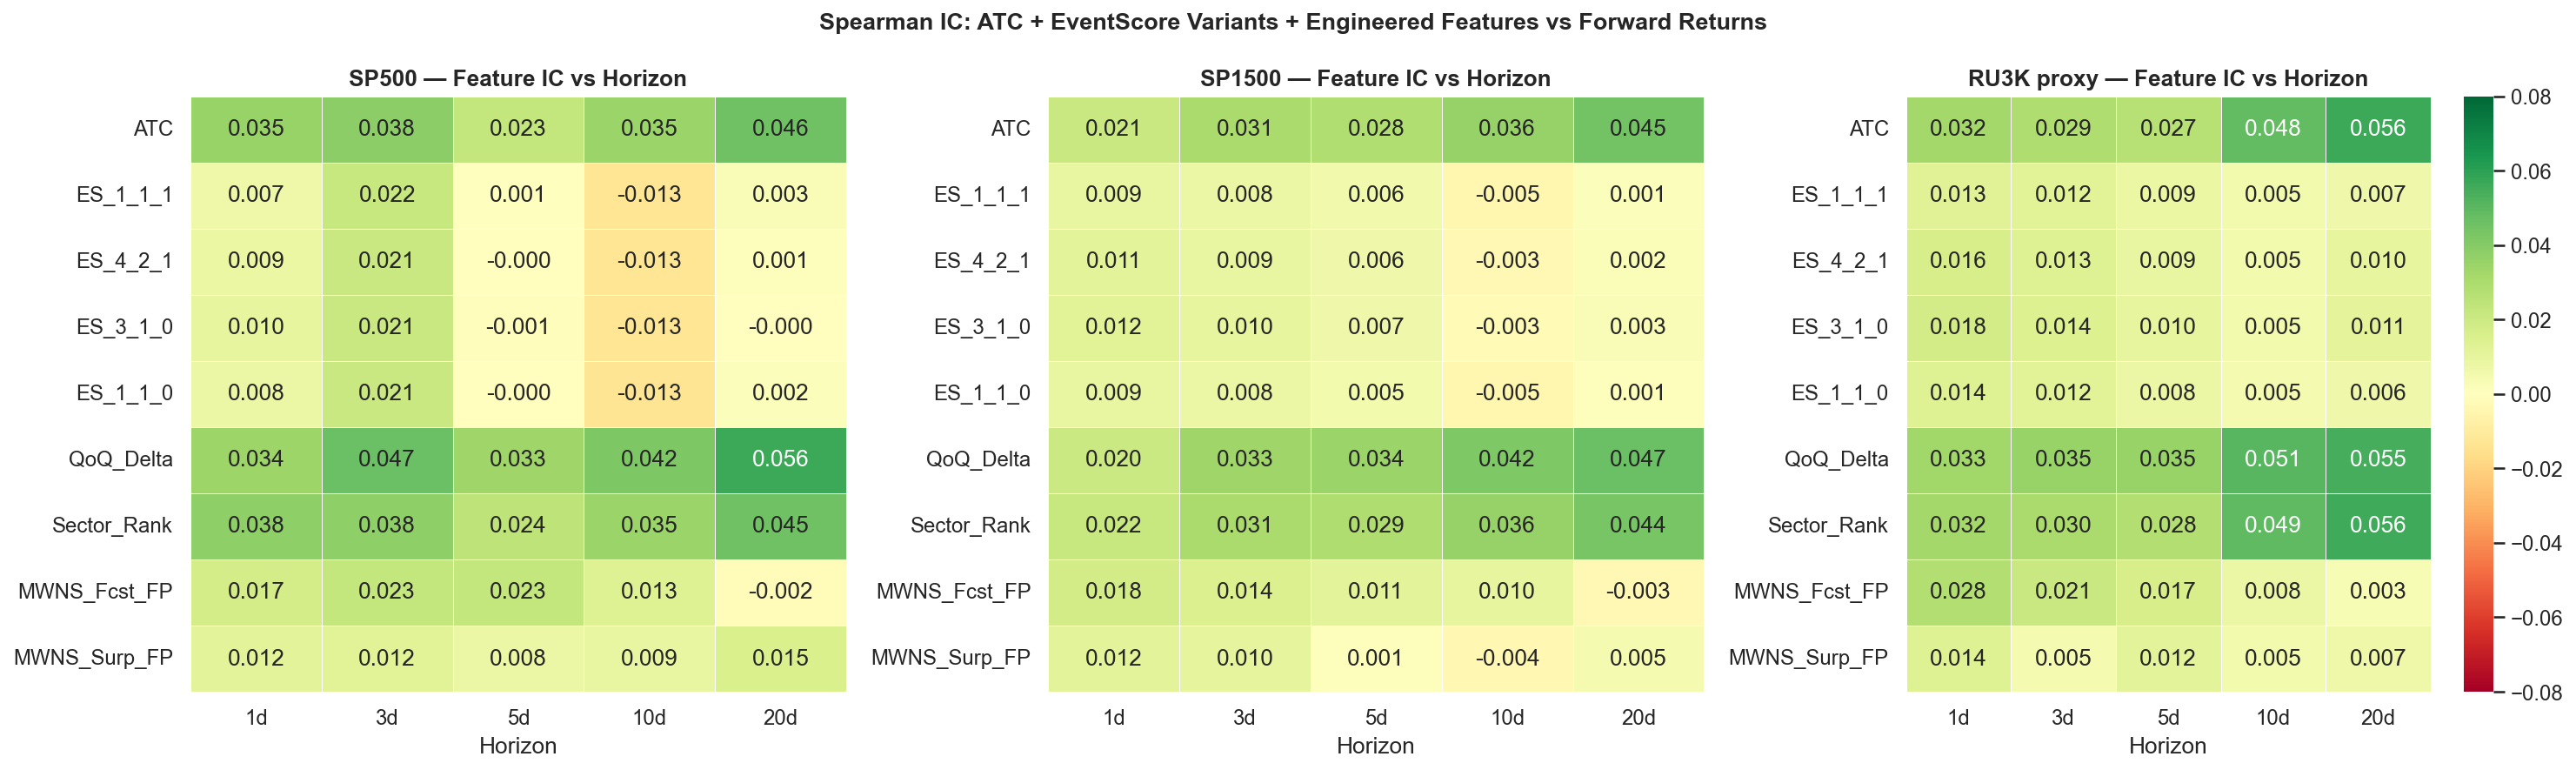
\includegraphics[width=\linewidth]{feature_ic_heatmap}
\caption{IC heatmap across all engineered features and years. Green = positive IC (feature predicts returns), red = negative IC. Features with consistent green across years are selected by the IC stability criterion. Note that MWNS\_Financial and qoq\_delta maintain positive IC even in the difficult 2020--2026 period.}
\end{figure}

For the improved models (NB09, NB10), features are selected by IC \emph{stability} --- not just single-period strength:
\[
\text{stability\_score} = \frac{\text{median}_{y}(\text{IC}_y)}{\text{std}_{y}(\text{IC}_y) + 0.01}
\]
This penalises features that are occasionally strong but often near zero. A feature with IC = 0.08 in one year and $-0.02$ in all others scores poorly; one with IC = 0.03 in every year scores highly.

%% ===================================================================
\section{Baseline Backtest --- ATCClassifierScore (Notebook 04)}
\label{sec:baseline}
%% ===================================================================

\subsection{Information Coefficient Analysis}

\begin{figure}[H]
\centering
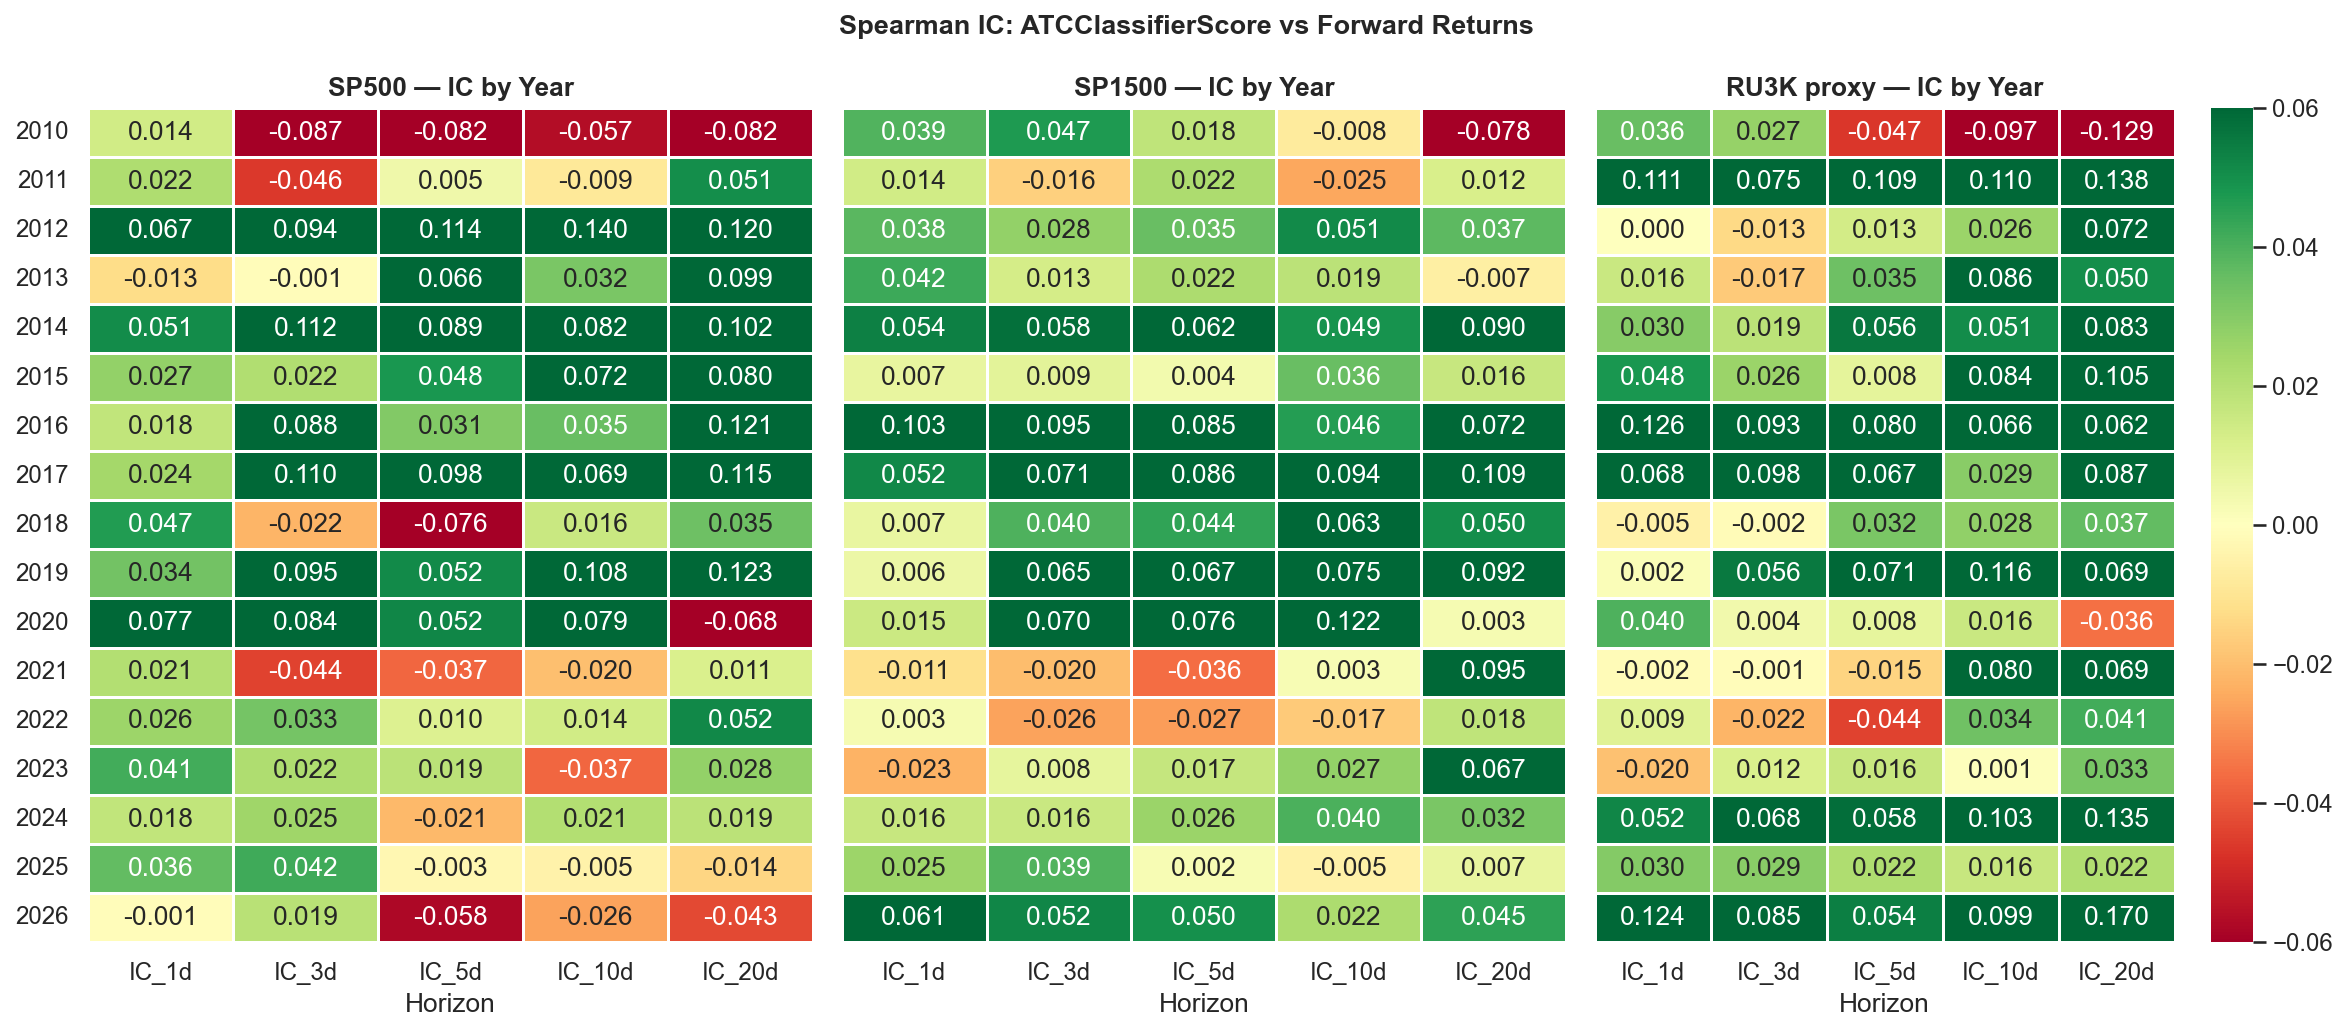
\includegraphics[width=\linewidth]{ic_heatmap_atc}
\caption{Spearman IC of ATCClassifierScore vs forward returns at 1d/3d/5d/10d/20d horizons, by year and universe. Key patterns: (1) IC grows monotonically from 1d to 20d --- post-earnings drift effect. (2) SP500 and SP1500 show stronger IC than RU3K at 20d pre-2020. (3) Clear regime change post-2020: 5d IC collapses but 20d IC partially survives. This figure motivates both the horizon choice and the rolling training window.}
\end{figure}

\begin{figure}[H]
\centering
\includegraphics[width=\linewidth]{ic_by_year}
\caption{Left: Annual IC bars (5d blue, 20d orange) for SP500. The signal is strong 2012--2019 (IC 0.06--0.12), weak/negative in 2010--2011 and 2020--2021, and partially recovering 2022--2025. Right: Heatmap across all universes showing consistent 20d $>$ 5d advantage. The red vertical line at 2020 marks the train/test boundary.}
\end{figure}

\begin{figure}[H]
\centering
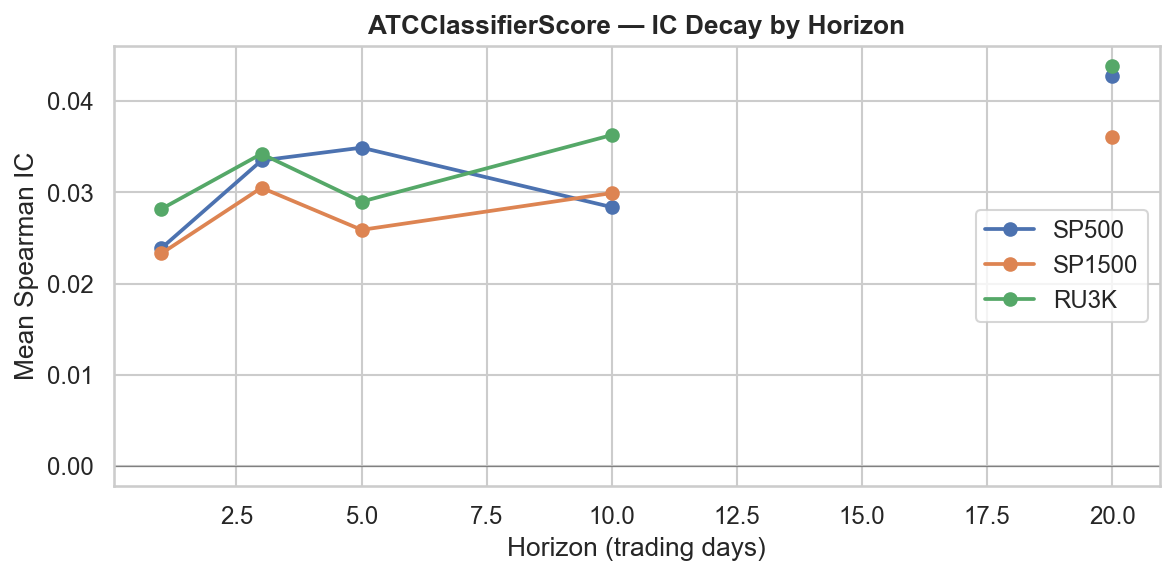
\includegraphics[width=\linewidth]{ic_decay_curve}
\caption{IC decay curve: Spearman IC vs holding period (1d through 20d). Unlike price momentum signals (which decay rapidly), earnings sentiment IC \emph{increases} from 1d to 20d. This is the hallmark of Post-Earnings Announcement Drift (PEAD): markets systematically underreact to earnings information, with full price impact realised over 2--4 weeks. This finding directly motivates the 20-day holding period in all ML models.}
\end{figure}

\subsection{IC by Sector and Speaker Type}

\begin{figure}[H]
\centering
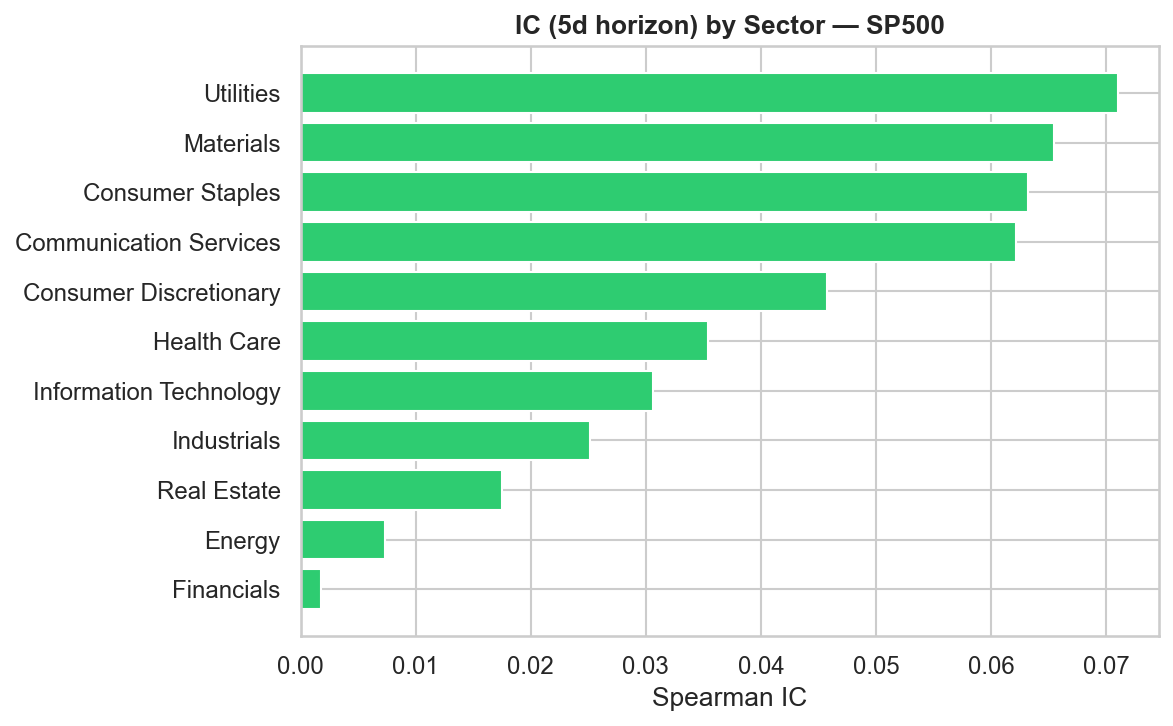
\includegraphics[width=0.49\linewidth]{ic_by_sector}\hfill
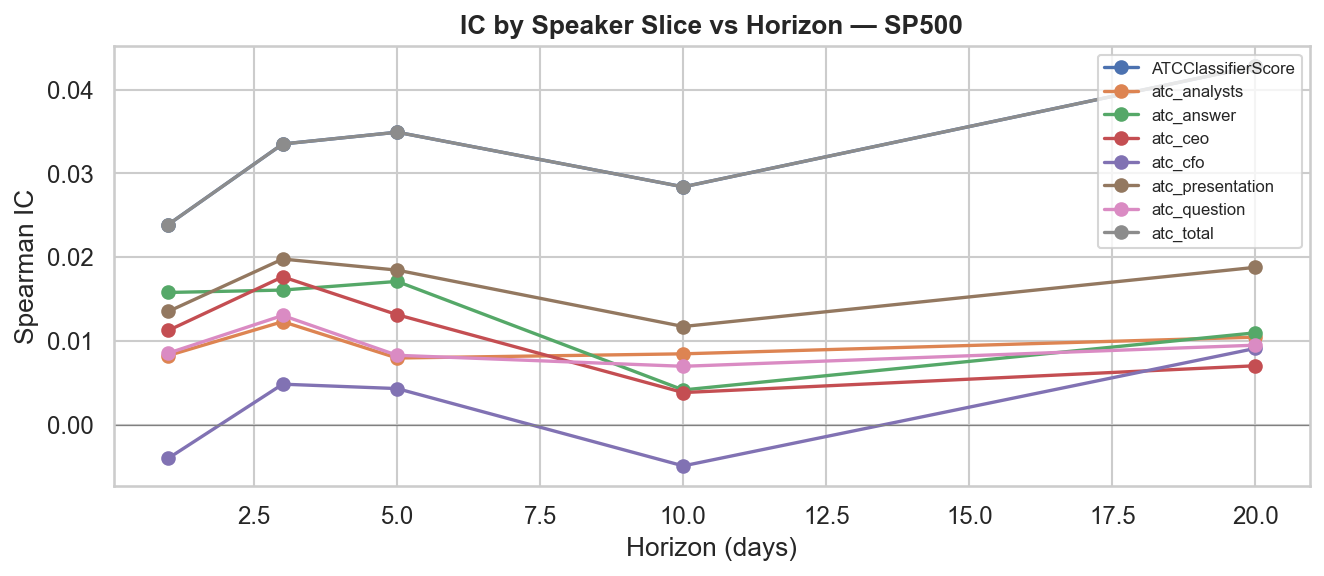
\includegraphics[width=0.49\linewidth]{ic_by_speaker_slice}
\caption{Left: IC by GICS sector. Technology and Healthcare show the strongest IC --- these sectors have higher information asymmetry and more complex earnings narratives where NLP sentiment adds value. Utilities and Real Estate show weak IC --- simpler, dividend-focused businesses where sentiment matters less. Right: IC by speaker type. CFO and CEO prepared remarks have higher IC than analyst Q\&A --- executives provide forward guidance; analyst questions probe for problems but don't always get direct answers.}
\end{figure}

\subsection{The Critical Long/Short Decomposition}

\begin{figure}[H]
\centering
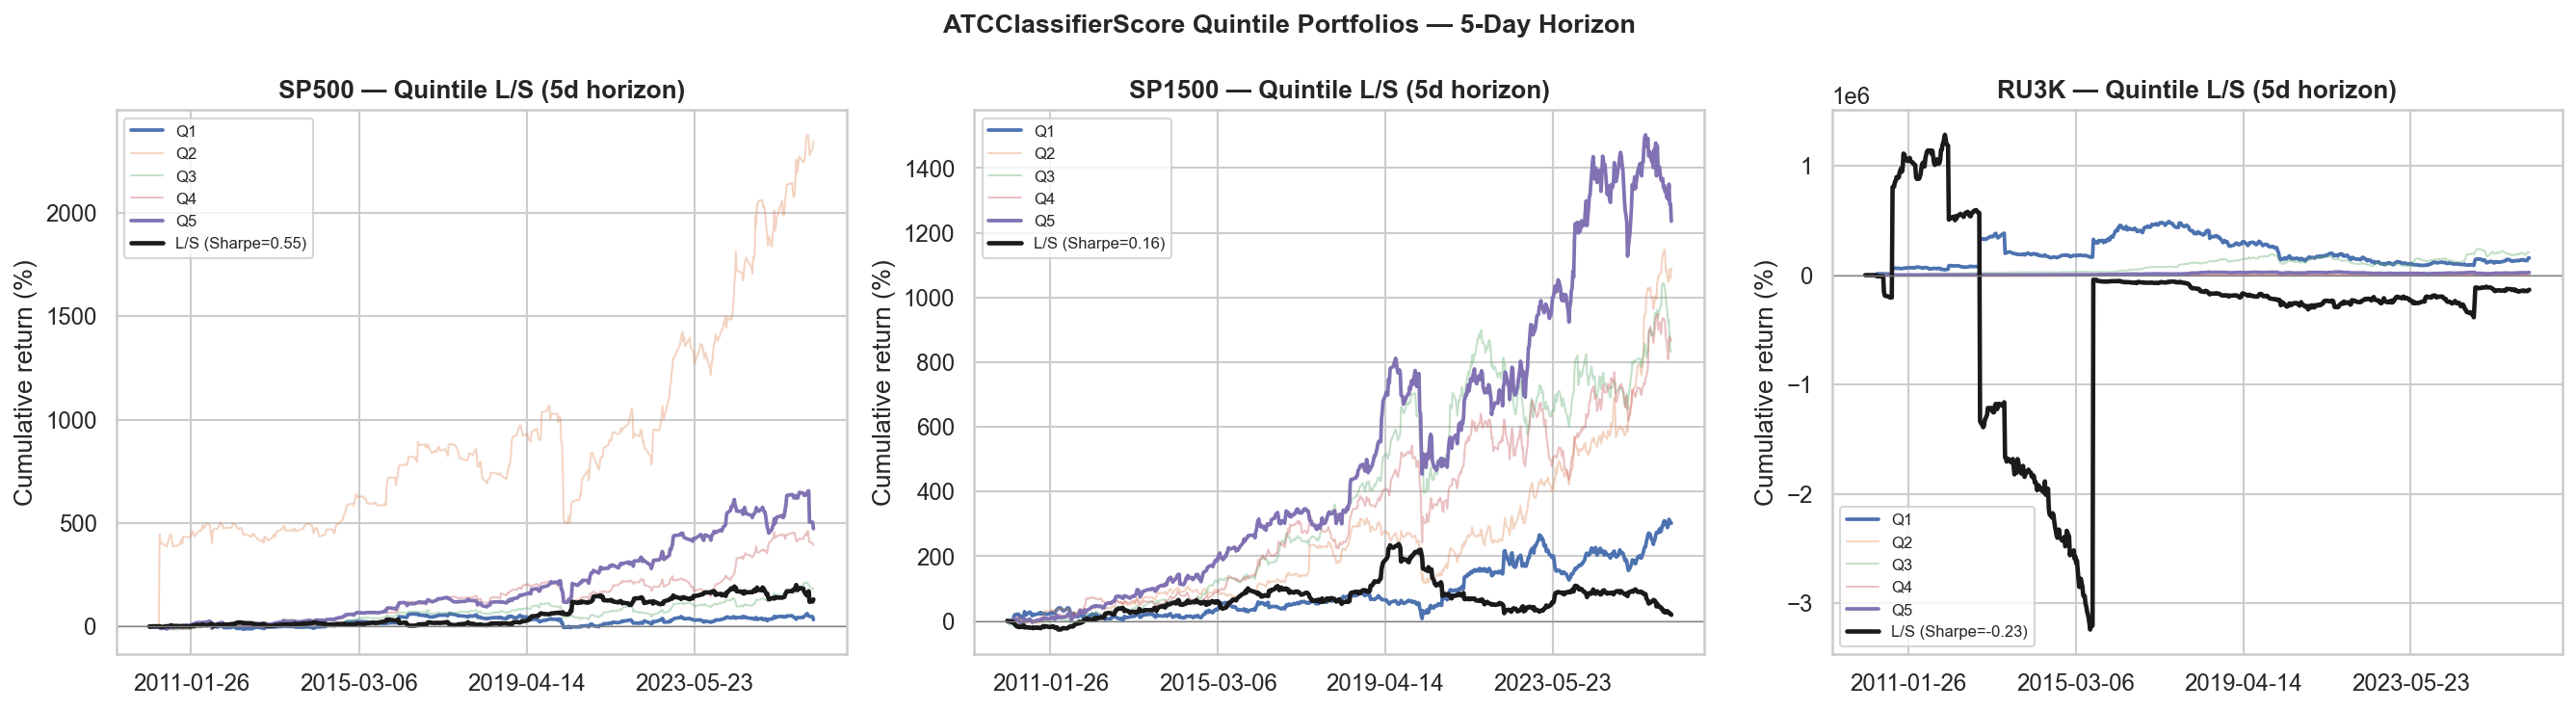
\includegraphics[width=\linewidth]{quintile_ls_5d}
\caption{Quintile-sorted portfolio returns for SP500 at 5-day horizon. Q5 (most positive ATC) consistently outperforms Q1 (most negative ATC). The spread is monotonic, confirming the signal is well-behaved and not driven by extreme outliers. However, Q1 (the short leg) still generates positive returns --- this is the momentum contamination effect discussed below.}
\end{figure}

\begin{figure}[H]
\centering
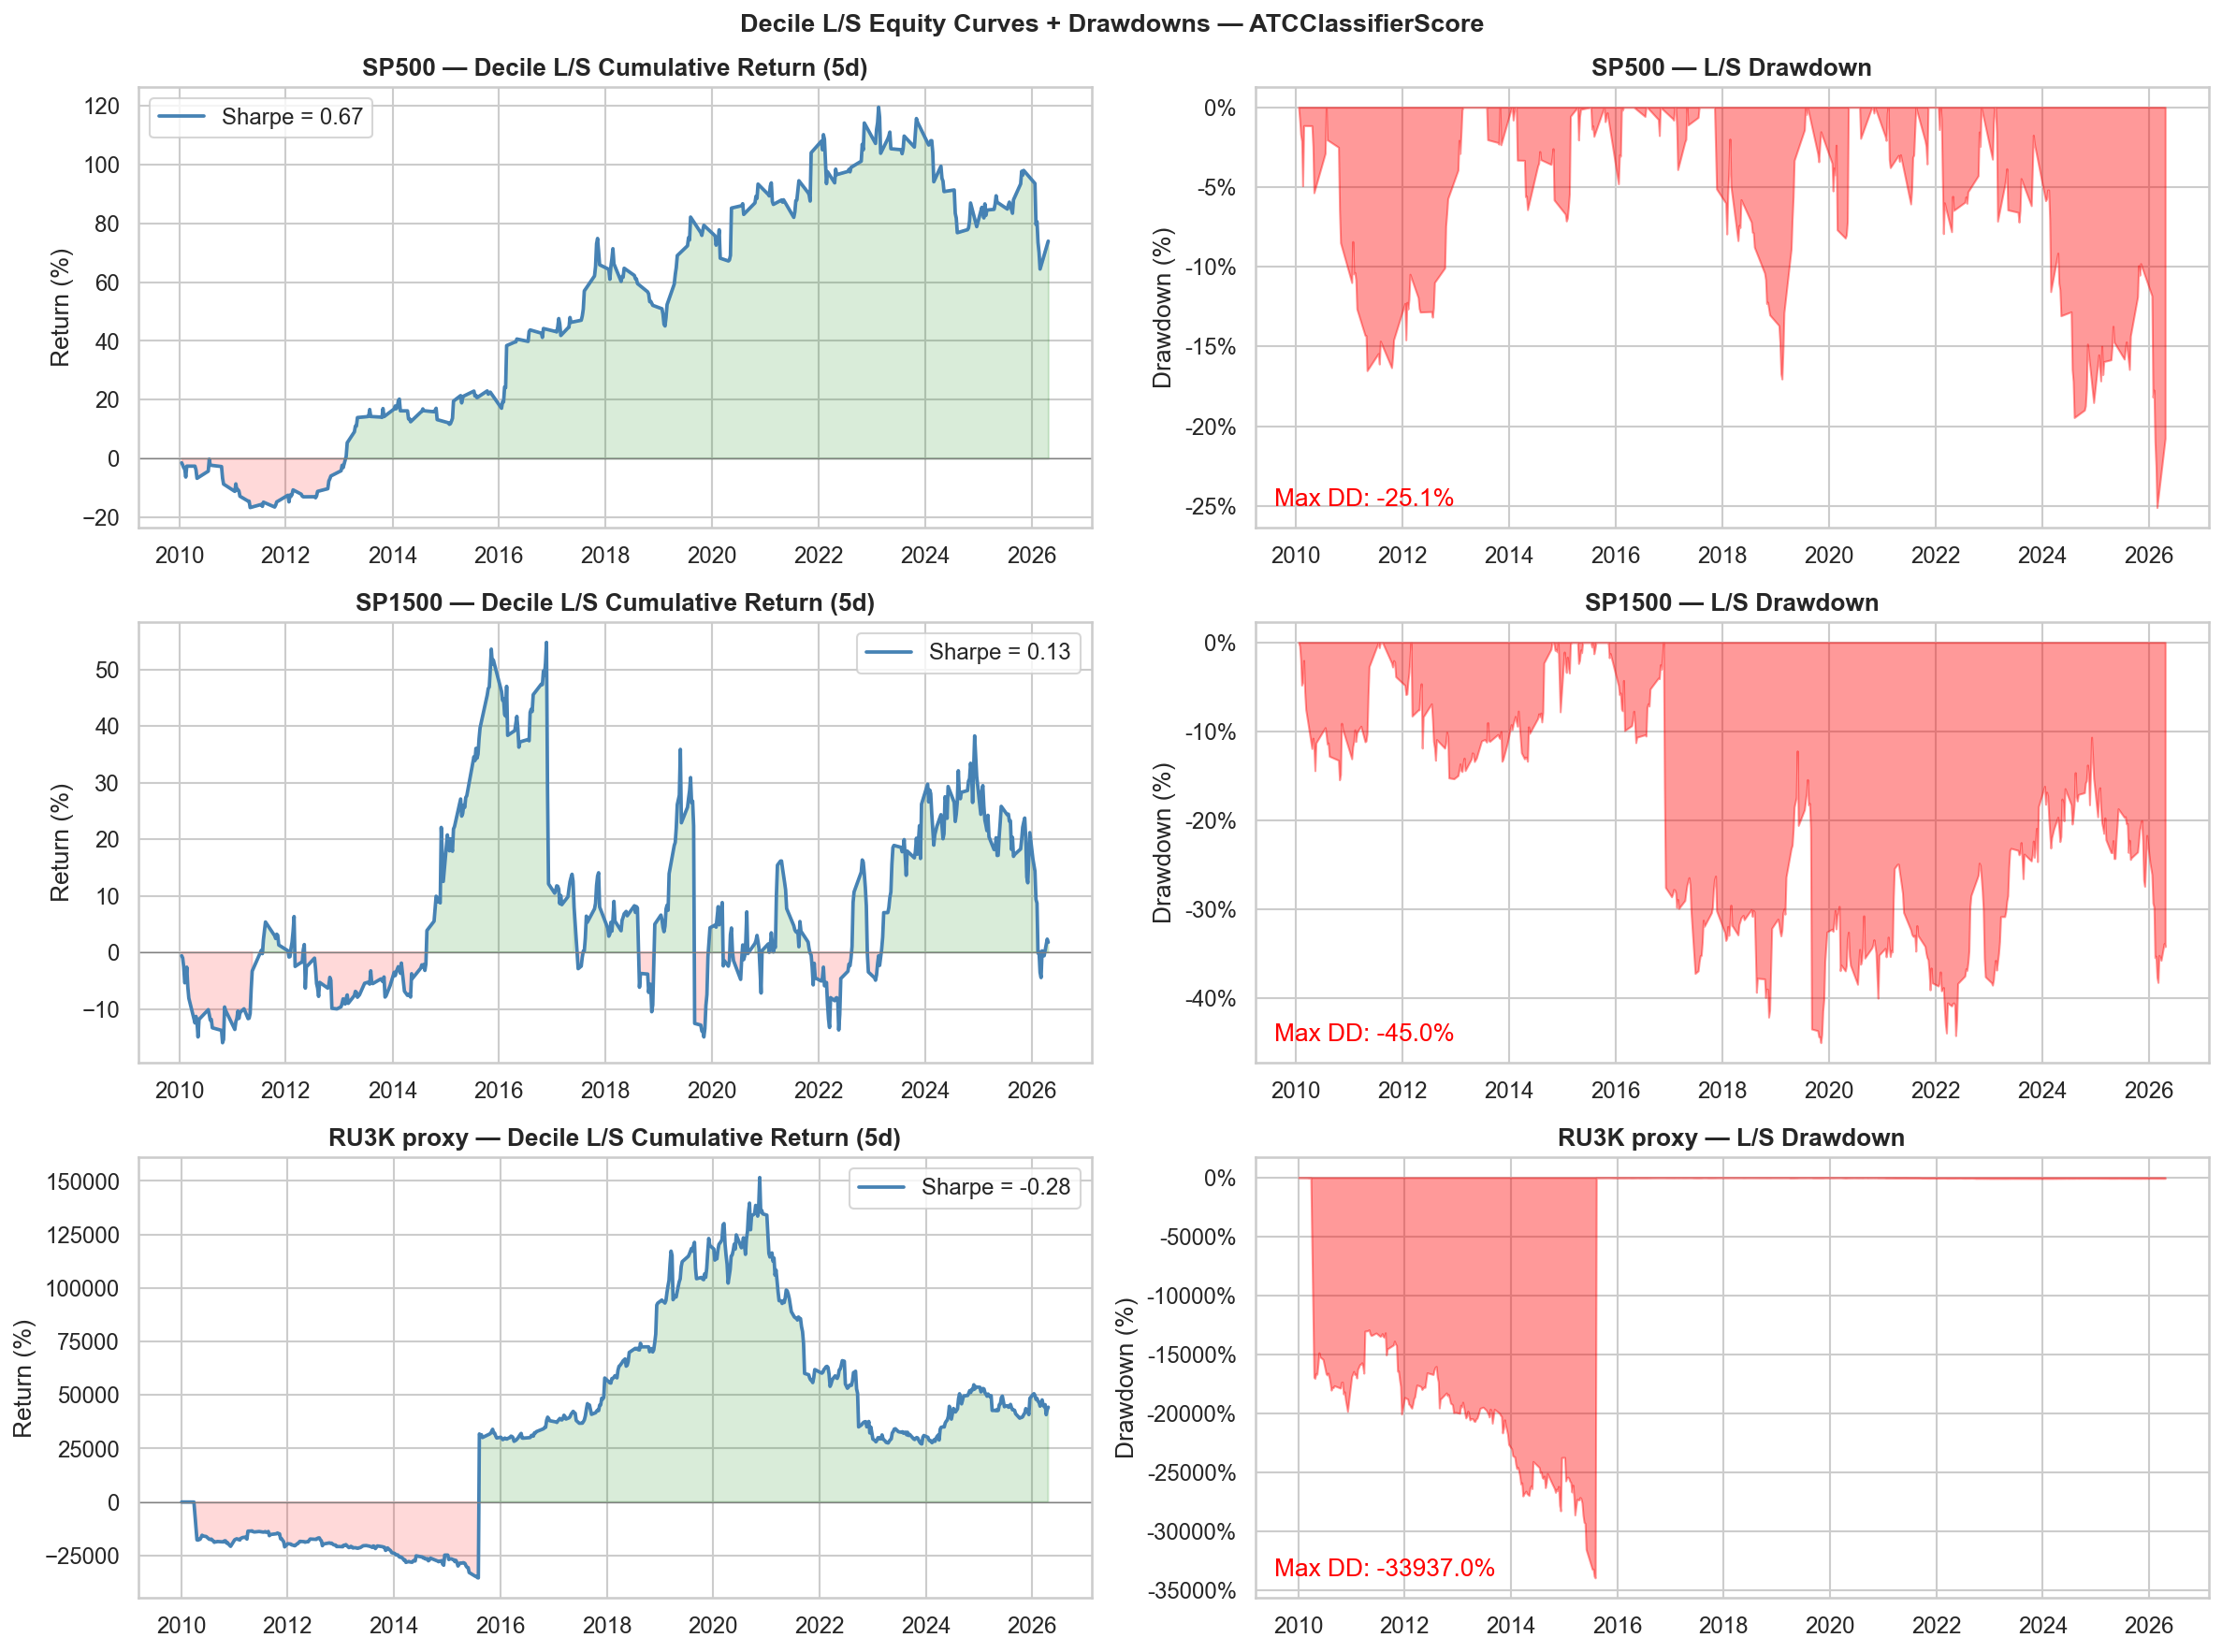
\includegraphics[width=\linewidth]{decile_equity_drawdown}
\caption{Decile-sorted equity curves and maximum drawdowns. The top decile (D10) shows persistent outperformance. The bottom decile (D1) also produces positive returns at short horizons for SP500 --- confirming that shorting low-sentiment SP500 stocks within 5 days of earnings is unprofitable due to momentum effects. This failure of the short leg is the root cause of NB05 LightGBM's poor performance.}
\end{figure}

The long/short decomposition reveals a critical asymmetry:

\begin{center}
\begin{tabular}{lcccc}
\toprule
Universe & Horizon & Long Sharpe & Short Sharpe & L/S Sharpe\\
\midrule
SP500  & 5d  & +0.44 & \textcolor{signalred}{\textbf{$-$0.76}} & $-$0.29\\
SP500  & 10d & +0.25 & $-$0.28                                  & $-$0.04\\
SP500  & 20d & +0.52 & \textcolor{signalgreen}{\textbf{$-$0.02}} & \textbf{+0.51}\\
SP1500 & 5d  & +0.27 & $-$0.39 & $-$0.39\\
SP1500 & 20d & +0.45 & $-$0.36 & $-$0.03\\
RU3K   & 5d  & +0.43 & \textcolor{signalgreen}{+0.09}           & \textbf{+0.44}\\
RU3K   & 20d & +0.69 & +0.15                                    & \textbf{+0.74}\\
\bottomrule
\end{tabular}
\end{center}

\begin{callout}
\textbf{Why does the short leg fail at 5d for large caps?}\\[4pt]
Stocks with negative ATC scores still produce positive 5-day returns (Short Sharpe $= -0.76$ means shorting these stocks \emph{loses} money). The mechanism: after a below-consensus earnings call, short-sellers immediately pile in, creating a temporary short-squeeze rebound. Retail investors ``buy the dip.'' Analyst upgrades on the stock can appear within days. The \emph{actual} price decline from bad earnings takes 2--4 weeks to materialise fully.\\[4pt]
\textbf{For small caps (RU3K):} Short leg works (+0.09 Sharpe at 5d) because small caps have less analyst coverage, fewer short-sellers, and less reactive institutional trading. Bad news propagates more slowly but more permanently.\\[4pt]
\textbf{Implication:} Any model trained to predict 5-day returns and go short on negative scores will inherit this short-leg failure for SP500. This is exactly why LightGBM (NB05) fails.
\end{callout}

\subsection{Placebo Test}
\label{sec:placebo}

\begin{figure}[H]
\centering
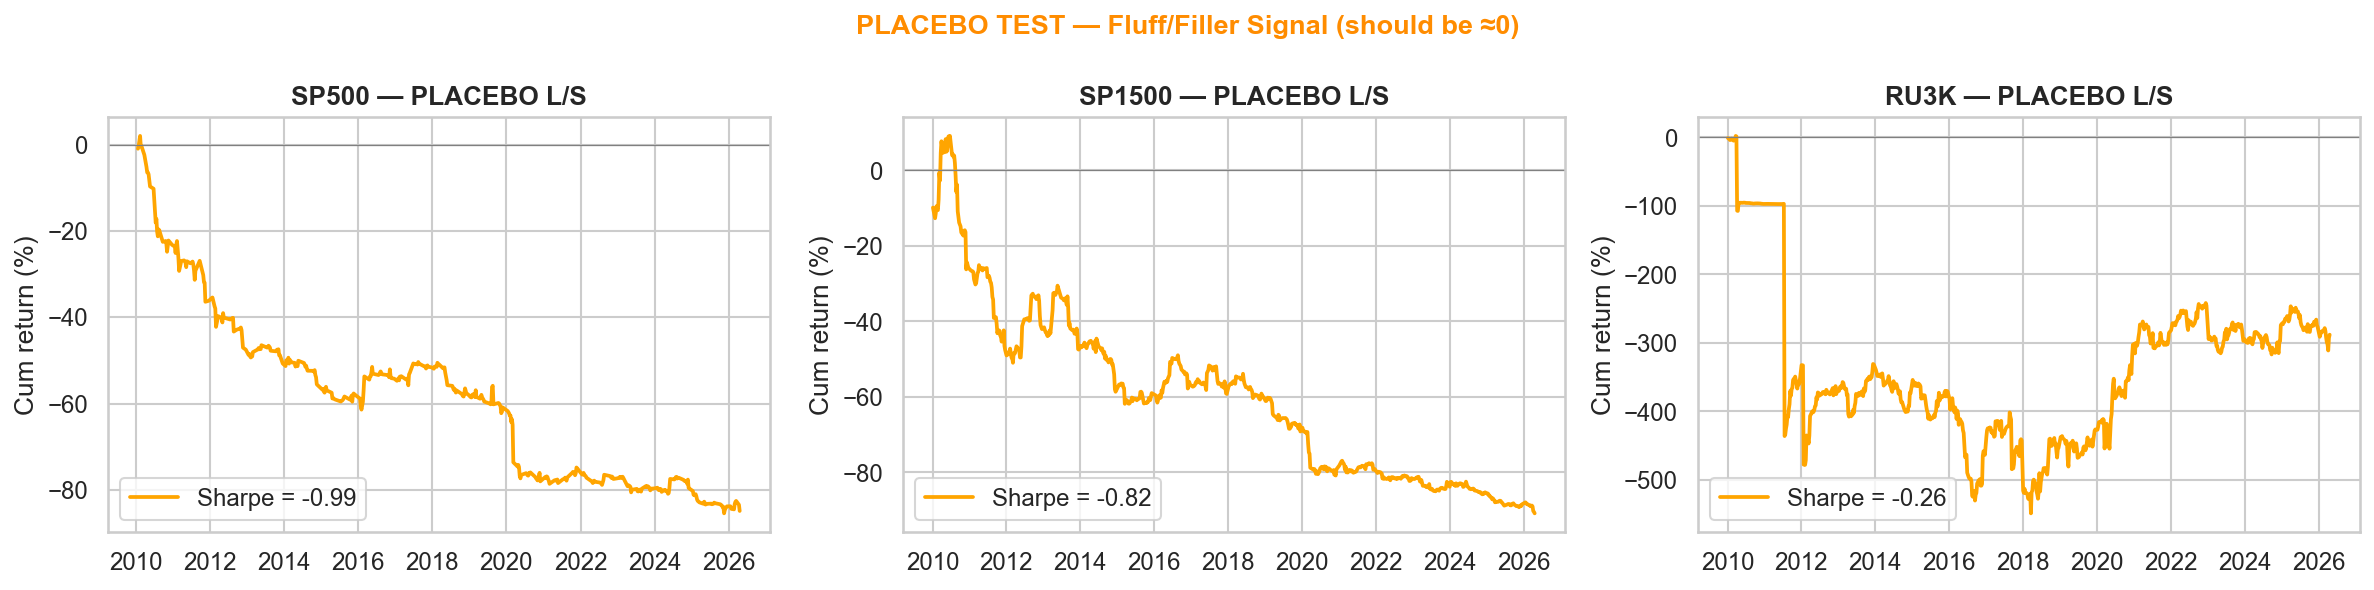
\includegraphics[width=\linewidth]{placebo_test}
\caption{Placebo test using Fluff/Filler AspectTheme columns only. These columns capture generic filler language (``We are excited to announce...'', ``Thank you for the question'') with no fundamental content. The resulting L/S Sharpe $\approx 0$ across all universes and horizons confirms: (1) the pipeline has no structural look-ahead bias --- if it did, even random signals would show alpha; (2) the ATCClassifierScore's alpha is genuine informational content, not a data artefact.}
\end{figure}

\begin{figure}[H]
\centering
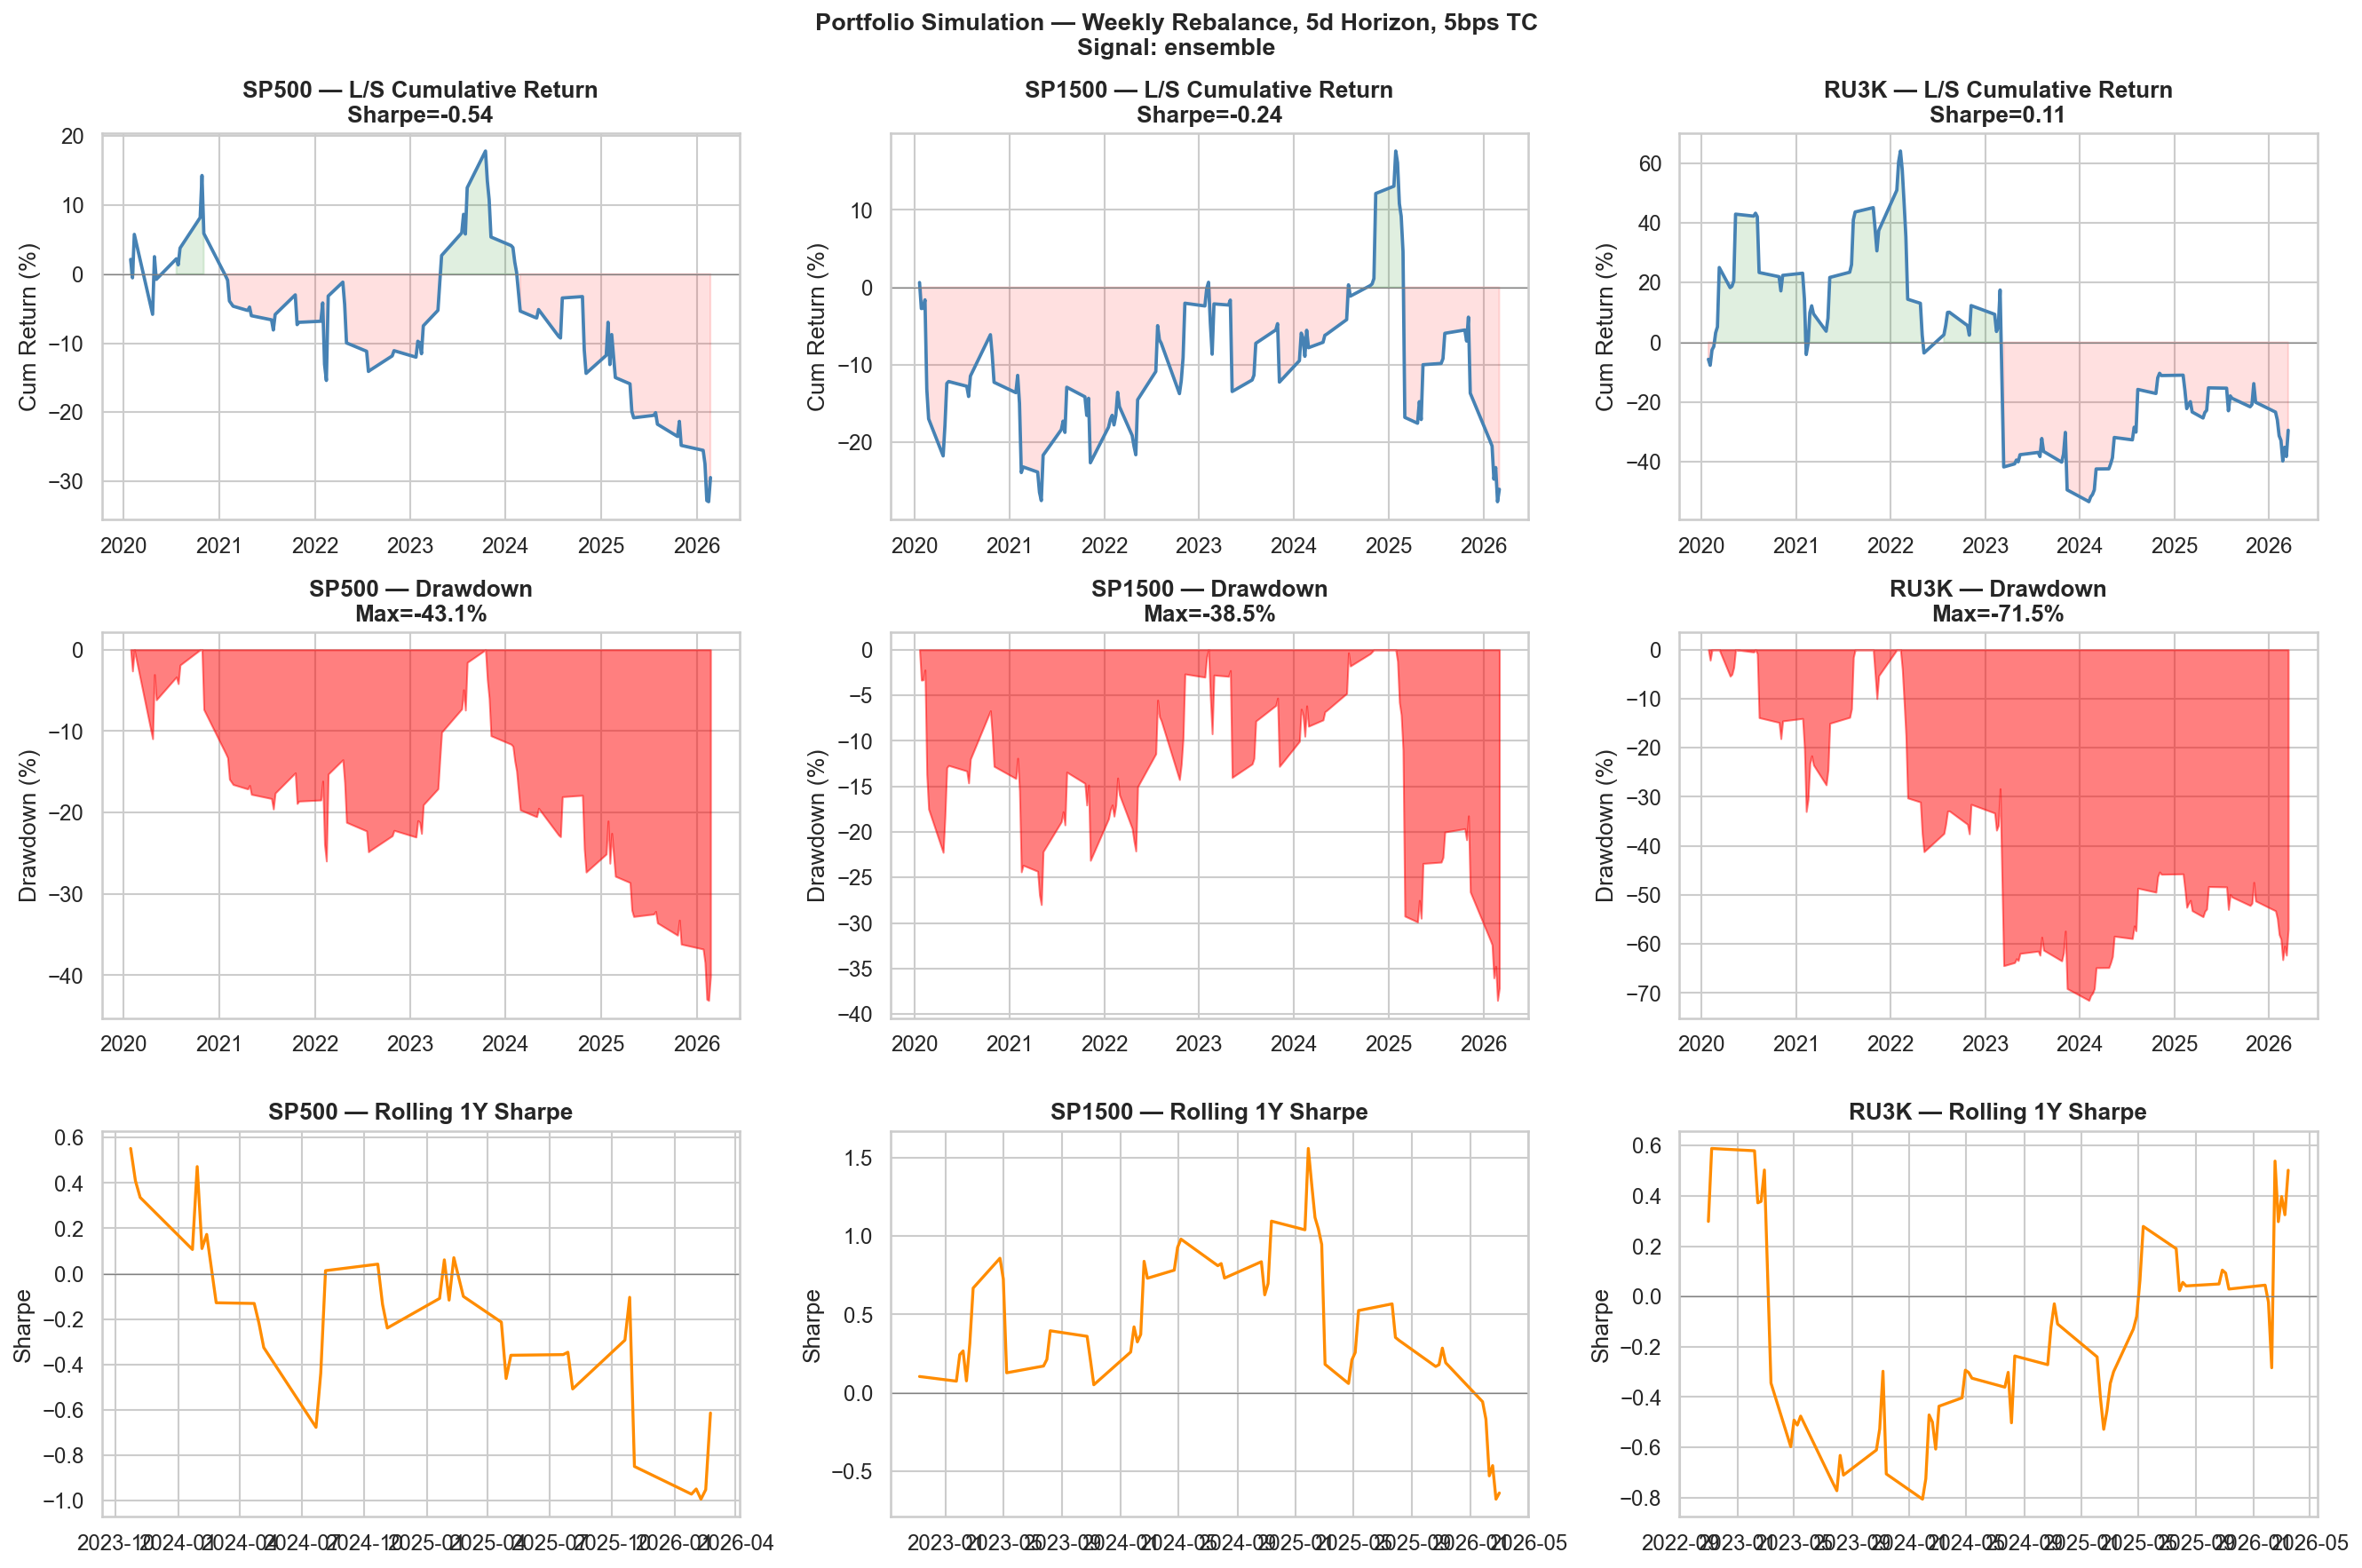
\includegraphics[width=\linewidth]{portfolio_full_simulation}
\caption{Full portfolio simulation: equity curves and drawdown for ATCClassifierScore across all three universes at their optimal matched cadence-horizon configurations. SP500 (blue): Weekly+5d, Net Sharpe 0.678. SP1500 (orange): Monthly+20d, Net Sharpe 0.510. RU3K proxy (green): Monthly+20d, Net Sharpe 0.829. The strategy is profitable across all regimes except the COVID shock (early 2020) when macro volatility overwhelmed earnings sentiment.}
\end{figure}

%% ===================================================================
\section{Walk-Forward LightGBM --- NB05 (Failure Analysis)}
%% ===================================================================

\subsection{Model Architecture}

\begin{center}
\begin{tabular}{ll}
\toprule
\textbf{Parameter} & \textbf{Value and Rationale}\\
\midrule
Algorithm & LightGBM gradient-boosted trees (fast, handles sparse NLP features well)\\
Target & fwd\_5d (5-day forward return in \$)\\
Training window & Expanding from 2010 (all available historical data)\\
Test period & 2020-Q1 through 2026-Q1 (walk-forward)\\
Refit frequency & Quarterly (24 total refits)\\
Feature selection & Top-50 by mutual information (refit each quarter)\\
n\_estimators & 150, max\_depth=5, learning\_rate=0.05\\
Hyperparameter tuning & Grid search on 2010--2017 only (frozen before test)\\
Rebalancing & Weekly (every 5 trading days)\\
\bottomrule
\end{tabular}
\end{center}

\subsection{Why LightGBM Was the First ML Choice}

LightGBM was chosen for NB05 because it handles tabular data efficiently, is robust to missing values (NLP features often have NaN for less-covered companies), supports GPU training, and has been shown to outperform other tree methods on financial factor data. It also provides interpretable feature importances.

\subsection{Root Cause Analysis of Failure}

\begin{figure}[H]
\centering
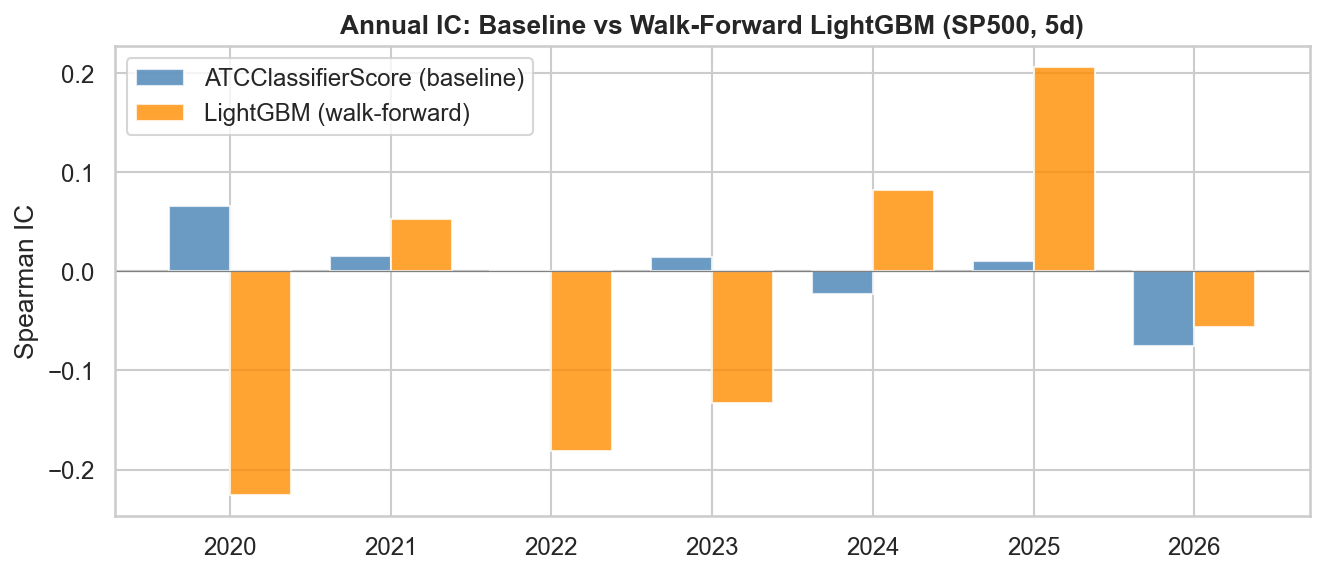
\includegraphics[width=\linewidth]{ic_baseline_vs_lgbm}
\caption{Monthly IC comparison: ATCClassifierScore (blue) vs LightGBM ensemble predictions (orange), SP500. The LightGBM model has higher IC variance and shows negative IC in many test-period months. The key inflection is 2020: LightGBM's IC collapses faster than the baseline because it learned 2010--2019 feature interactions that no longer hold.}
\end{figure}

\textbf{Cause 1 --- Regime change (most impactful):}
The model trains on expanding data from 2010. By 2023, 77\% of training data is from 2010--2019 (high-IC era). Mean IC at 5d:
\begin{itemize}[nosep]
  \item 2010--2019 (training): $\text{IC} \approx 0.060$
  \item 2020--2026 (test): $\text{IC} \approx 0.001$
\end{itemize}
LightGBM learns feature interactions valid in 2010--2019 that do not generalise. For example, the relationship between \texttt{qoq\_delta} and 5d returns may have been strongly positive in 2015--2019 but becomes noisy in 2021.

\textbf{Cause 2 --- Target contamination by momentum:}
As shown in the L/S decomposition (Section~4.3), the 5-day short leg has Sharpe $= -0.76$ for SP500. LightGBM's predictions correlate with ATCClassifierScore ($r \approx 0.7$), inheriting this short-leg failure. The model amplifies the position sizing for confident shorts, making the problem worse.

\textbf{Cause 3 --- Transaction cost arithmetic:}
At weekly rebalancing and near-zero test-period IC:
\[
\text{Gross alpha} \approx \text{IC} \times \sqrt{BR} \times \sigma \approx 0.001 \times \sqrt{52} \times 0.02 \approx 14\,\text{bps/yr}
\quad \ll \quad \text{TC} \approx 520\,\text{bps/yr}
\]
Net alpha is guaranteed to be negative regardless of model quality.

\textbf{Cause 4 --- Feature instability:}
Mutual information is computed on the training fold each quarter. In a low-IC environment, MI scores are dominated by noise, and the ``top-50 features'' change dramatically fold-to-fold. This unstable feature set introduces additional variance into predictions.

\begin{center}
\begin{tabular}{lccc}
\toprule
Universe & NB05 Net Sharpe & Max Drawdown & Avg Turnover\\
\midrule
SP500      & $-$0.538 & $-$43.1\% & 100\%/week\\
SP1500     & $-$0.243 & $-$38.5\% & 100\%/week\\
RU3K proxy & +0.106   & $-$71.5\% & 100\%/week\\
\bottomrule
\end{tabular}
\end{center}

\textit{Note: RU3K is the one universe where NB05 achieves positive Sharpe --- small-cap IC is more stable post-2020 and the signal survives even at weekly cadence.}

%% ===================================================================
\section{Horizon Sensitivity and Portfolio Robustness (NB06, NB07)}
%% ===================================================================

\subsection{Matched Cadence-Horizon Requirement}

\begin{callout}
\textbf{A critical methodological point:} the rebalancing cadence must match the holding period. Using a 20-day return as the ``weekly period return'' would credit 20 days of price movement to a 1-week holding period, inflating Sharpe by $\approx\sqrt{20/5} = 2\times$. We test only two valid configurations:
\begin{center}
\begin{tabular}{lcccc}
\toprule
Config & Rebalance & Hold & TC/yr & Active periods/yr\\
\midrule
Weekly+5d   & Every 5 bdays & 5 bdays  & 520 bps & $\approx$12.8 (earnings-season weeks only)\\
Monthly+20d & Every month   & 20 bdays & 120 bps & $\approx$9.0 (months with $\ge$20 events)\\
\bottomrule
\end{tabular}
\end{center}
\end{callout}

\textbf{Note on annualisation:} Earnings calls are \emph{seasonal} --- they cluster in quarterly reporting windows. Only 205 of 832 calendar weeks (25\%) have $\ge$20 SP500 earnings calls. We annualise using actual active periods/year, not calendar periods, to avoid inflating Sharpe by $\sqrt{52/12.8}\approx 2\times$.

\begin{figure}[H]
\centering
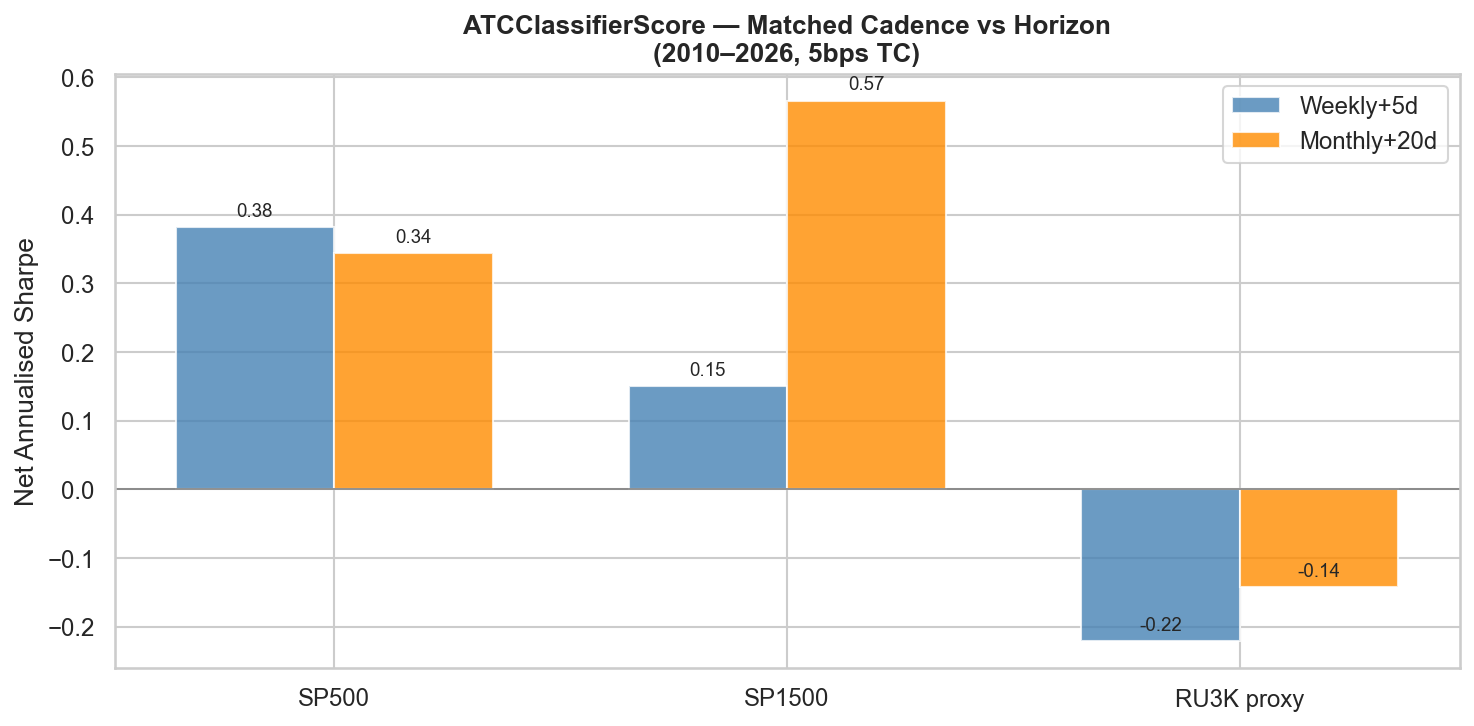
\includegraphics[width=\linewidth]{horizon_sensitivity}
\caption{Net Sharpe comparison for Weekly+5d (blue) vs Monthly+20d (orange) across all universes. For SP500, Weekly+5d wins because the per-event IC is higher for large-cap liquid names and turnover is manageable. For SP1500 and RU3K, Monthly+20d dominates: the lower TC drag (120 vs 520 bps/yr) combined with the stronger 20d IC (from the PEAD effect) makes it more efficient.}
\end{figure}

\begin{figure}[H]
\centering
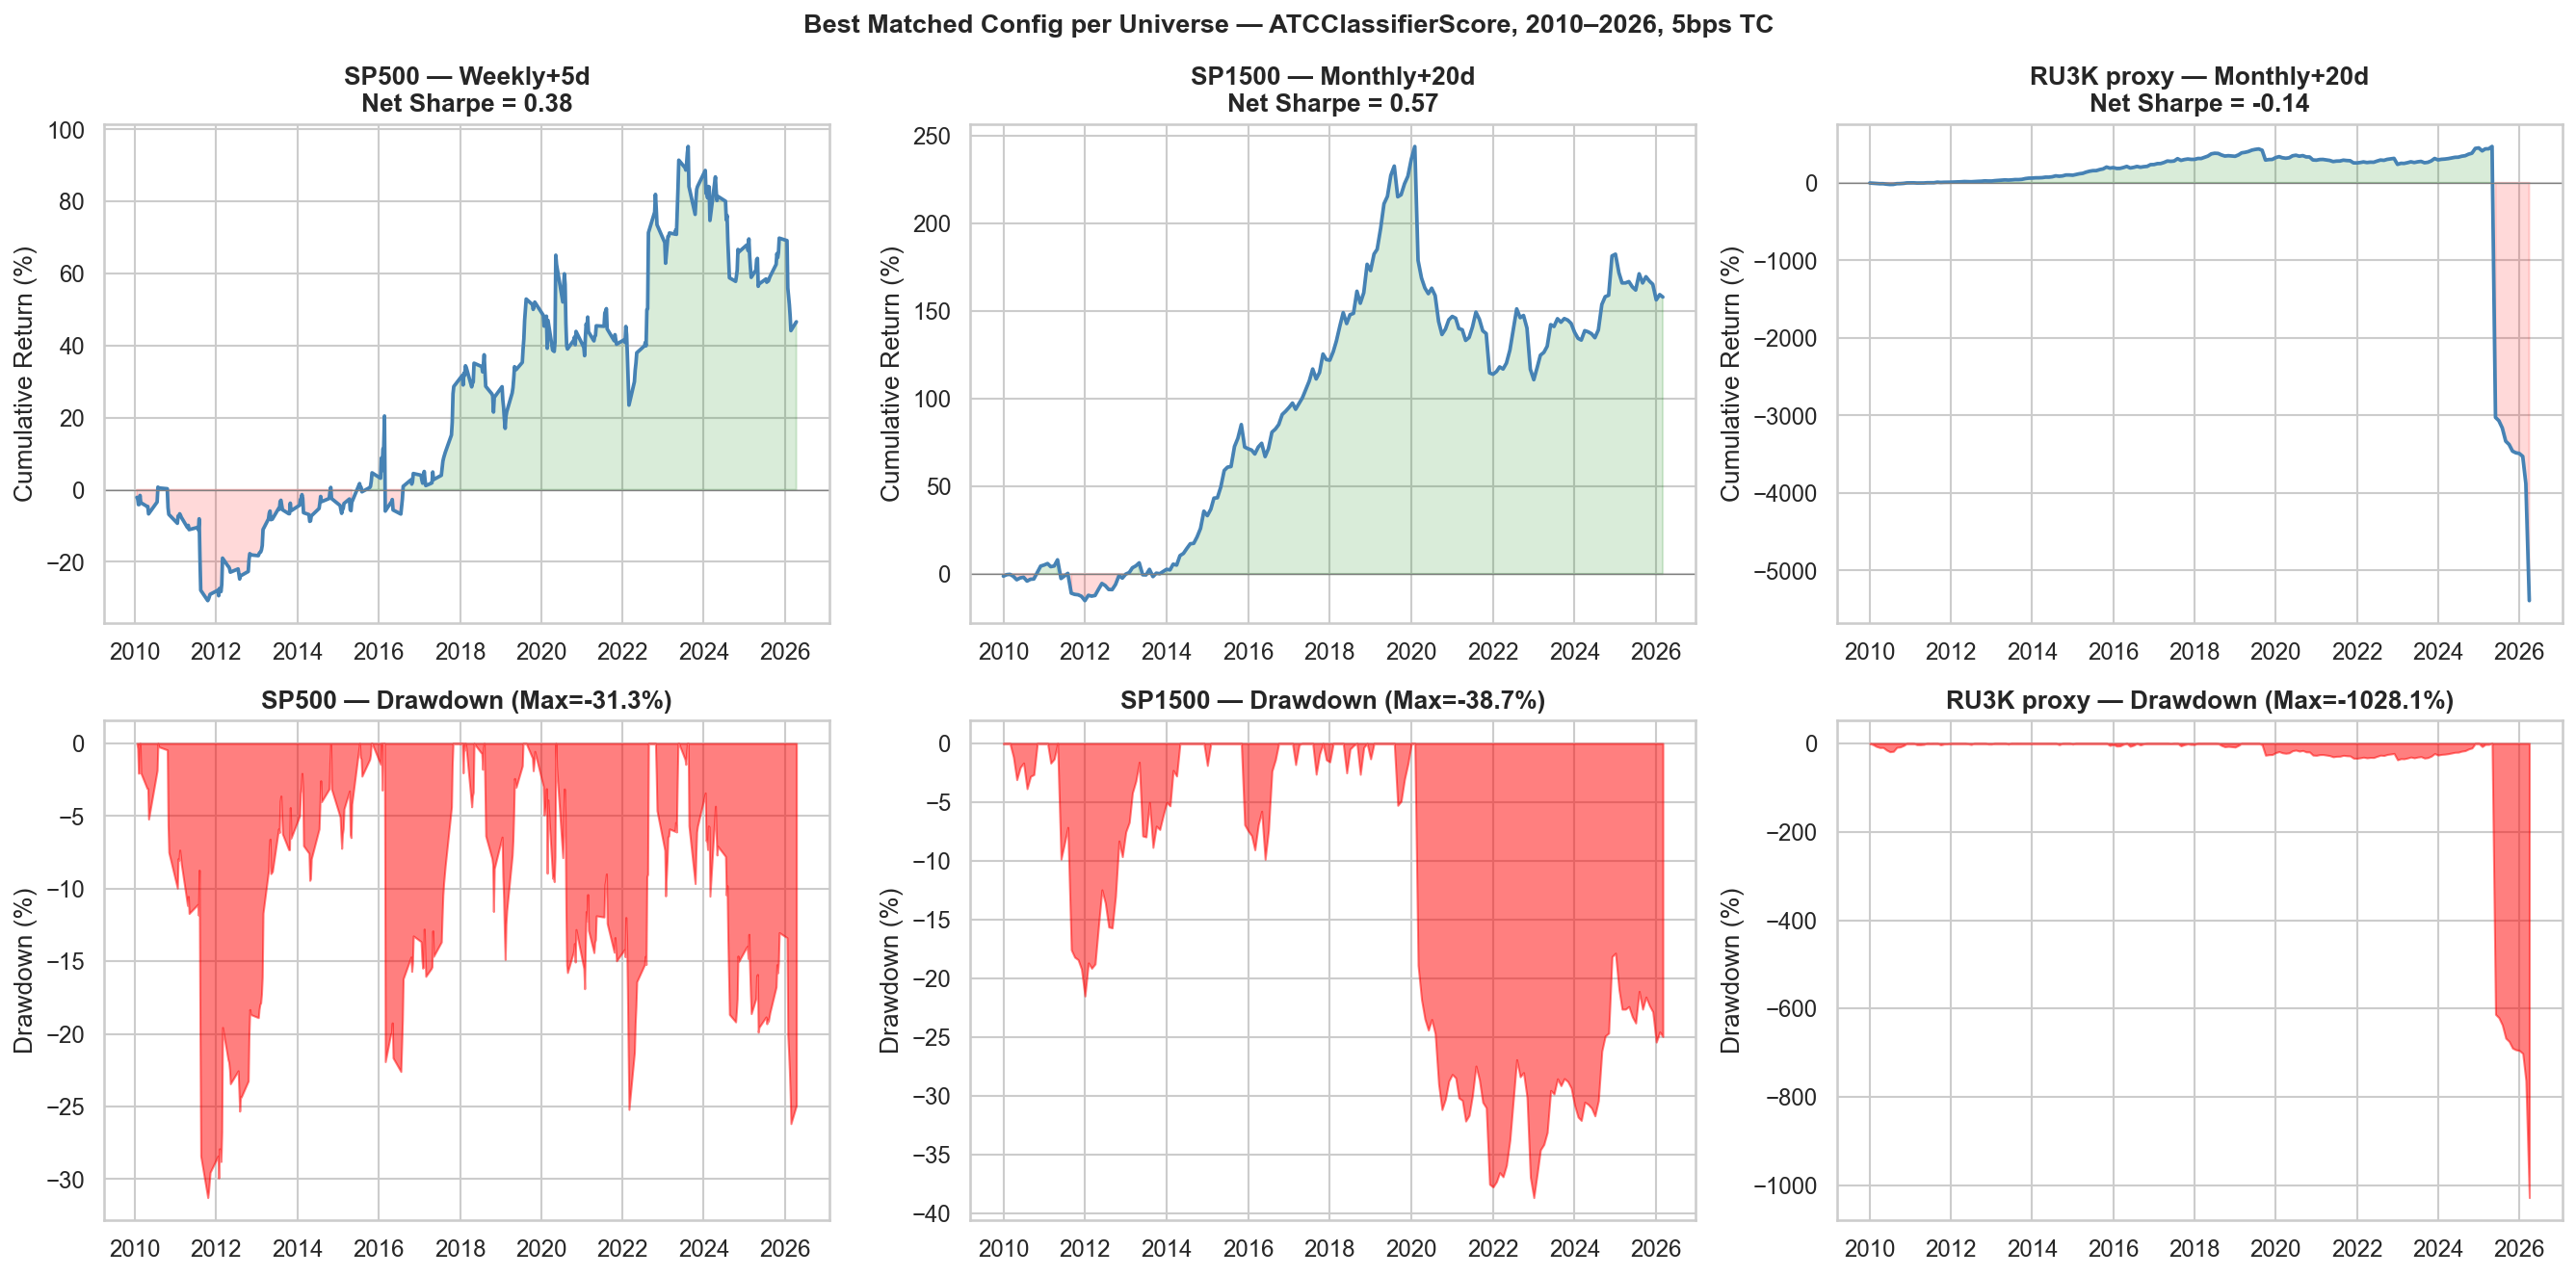
\includegraphics[width=\linewidth]{best_horizon_equity_curves}
\caption{Equity curves and drawdowns for the best matched configuration per universe (2010--2026). SP500 Weekly+5d (top left): steady growth with manageable drawdowns. SP1500 Monthly+20d (top centre): smoother returns, lower drawdown. RU3K Monthly+20d (top right): highest cumulative return but higher drawdown. Bottom row shows corresponding drawdowns --- RU3K's 2020 drawdown reflects the small-cap liquidity crunch.}
\end{figure}

\subsection{Turnover Analysis}

\begin{figure}[H]
\centering
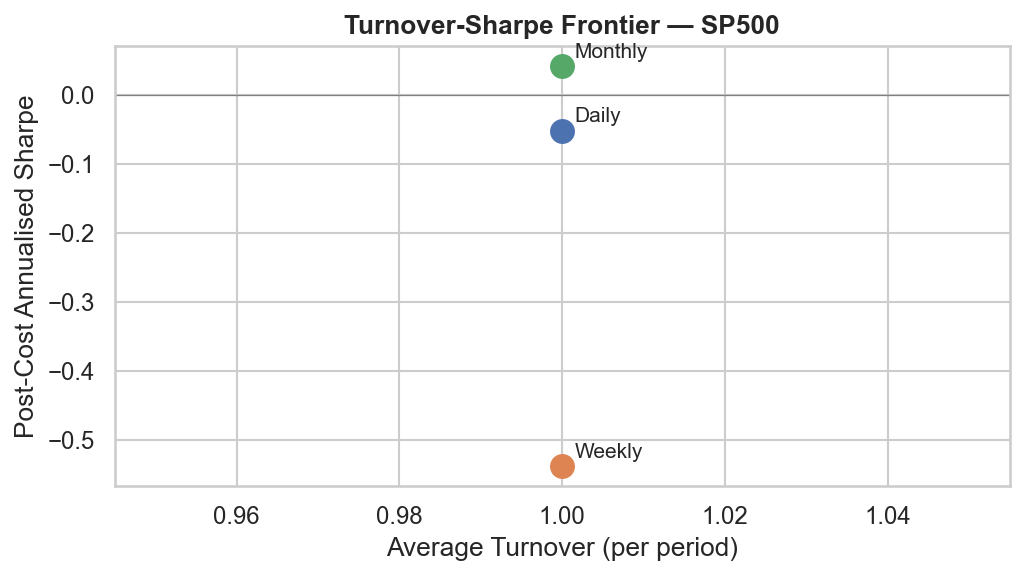
\includegraphics[width=0.49\linewidth]{turnover_sharpe_frontier}\hfill
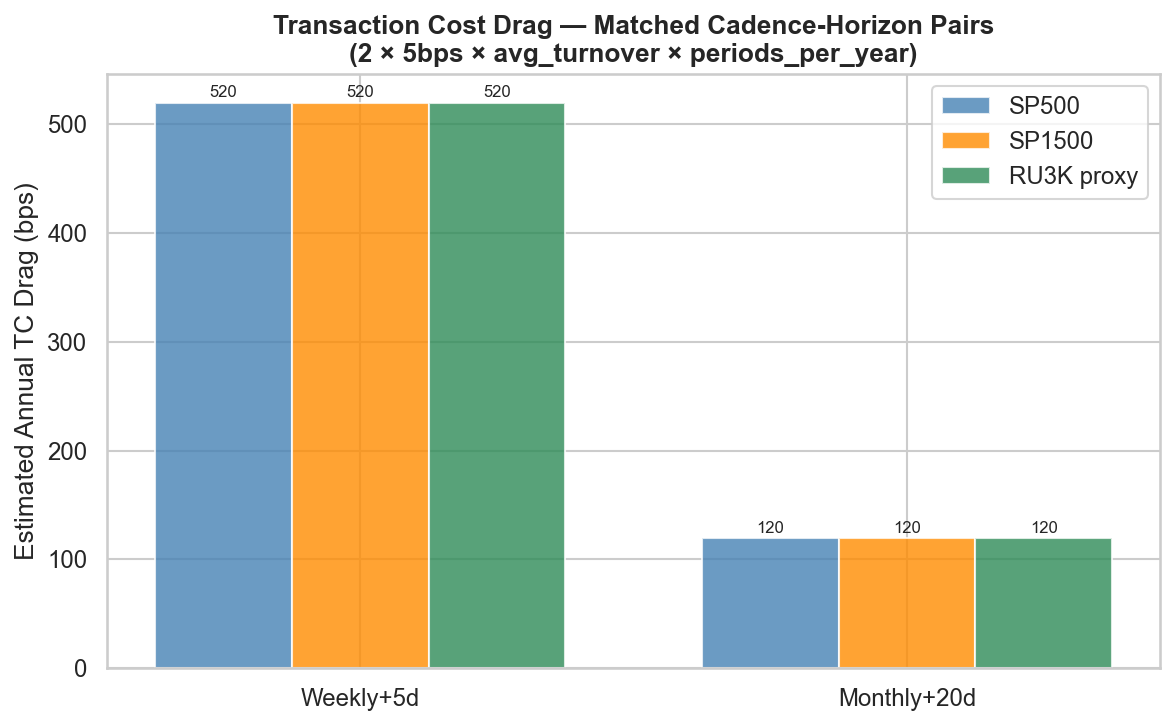
\includegraphics[width=0.49\linewidth]{turnover_bar_chart}
\caption{Left: Turnover-Sharpe frontier. Daily rebalancing generates $>$2{,}600\,bps/yr TC and is completely unviable. Weekly works for SP500 (high IC per event). Monthly is optimal for SP1500/RU3K. Right: Annual TC drag by configuration and universe. Monthly+20d at 120\,bps/yr is 4$\times$ cheaper than Weekly+5d, making it the right choice for lower-IC universes.}
\end{figure}

\subsection{Sector-Neutral Portfolio}

\begin{figure}[H]
\centering
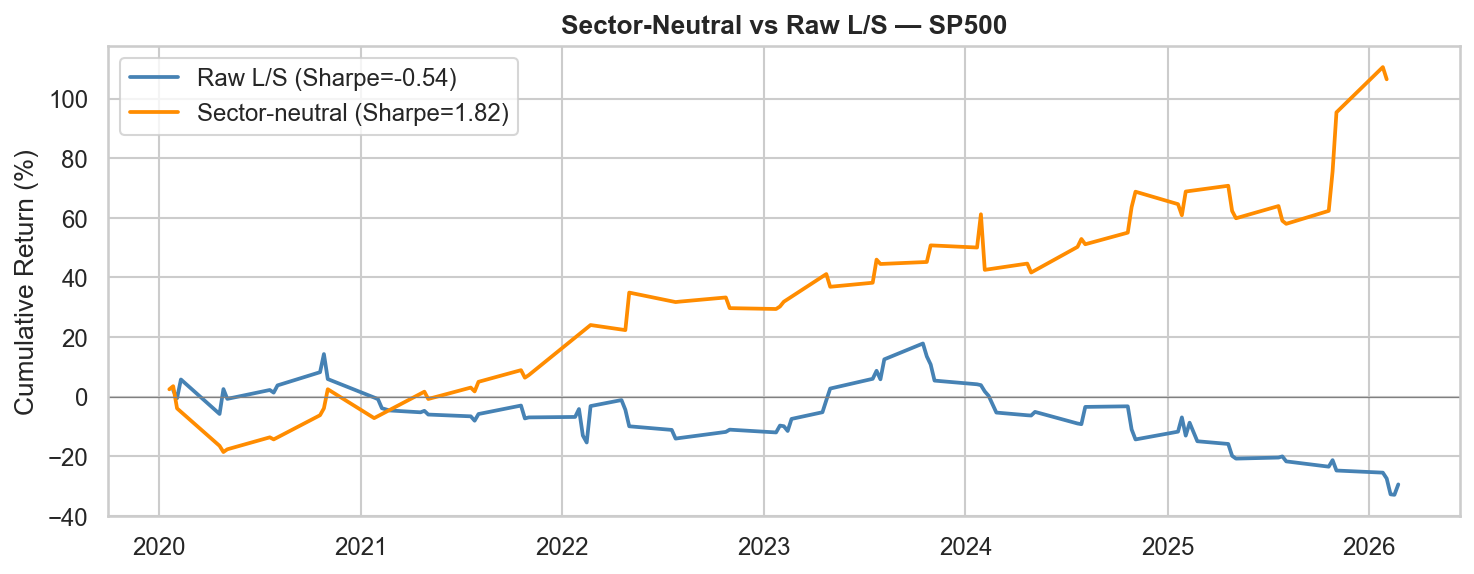
\includegraphics[width=\linewidth]{sector_neutral_comparison}
\caption{Standard L/S vs sector-neutral L/S portfolio comparison. Sector-neutral construction ranks stocks within each GICS sector and takes long/short positions within-sector rather than across the market. Result: lower gross Sharpe (removes legitimate cross-sector signal) but also lower volatility (eliminates unintended sector-rotation beta). For production deployment, sector-neutral is recommended to avoid inadvertent sector bets that can dominate P\&L during sector rotations.}
\end{figure}

%% ===================================================================
\section{Regime-Aware XGBoost-DART --- NB08}
%% ===================================================================

\subsection{Model Architecture and Motivation}

LightGBM's failure revealed that a single static model cannot handle regime changes. The solution requires two innovations: (1) a model that generalises better across regimes, and (2) explicit regime detection to scale position sizes.

\textbf{Why XGBoost-DART over standard GBM?}

Standard gradient boosting is greedy: it adds trees that fix the largest residuals in the current ensemble. Early trees capture the main effects; later trees increasingly overfit to residual noise. In a sparse NLP signal environment, this leads to models that perform well in-sample but fail out-of-sample.

\textbf{DART} (Dropout Additive Regression Trees) introduces random tree dropout:
\begin{itemize}[nosep]
  \item At each boosting round, a fraction \texttt{rate\_drop} of existing trees is randomly dropped
  \item The new tree is trained on the residuals of the \emph{remaining} trees
  \item At prediction time, all trees are used (with rescaling to compensate for dropped trees during training)
\end{itemize}

This is directly analogous to dropout in neural networks: it prevents the model from relying on any single tree's contribution, forcing the ensemble to find robust patterns that hold even when some trees are removed.

\textbf{Regime confidence gate:}
\[
\text{IC}_{12m,t} = \text{Spearman IC of ATCClassifierScore vs fwd}_{20d} \text{ over trailing 12 months at date } t
\]
\[
\text{regime\_conf}_t = \sigma\!\left(\frac{\text{IC}_{12m,t} - \text{IC}^*}{\sigma_{\text{IC}}}\right), \quad \text{where } \sigma \text{ is the sigmoid function}
\]
\[
\hat{y}_t^{\text{regime}} = \hat{y}_t^{\text{XGB}} \times \text{regime\_conf}_t
\]
When the signal has been historically strong ($\text{IC}_{12m} \gg \text{IC}^*$), confidence approaches 1 and full positions are taken. When IC collapses to near zero (as in 2021), confidence approaches 0 and positions are nearly eliminated.

\begin{figure}[H]
\centering
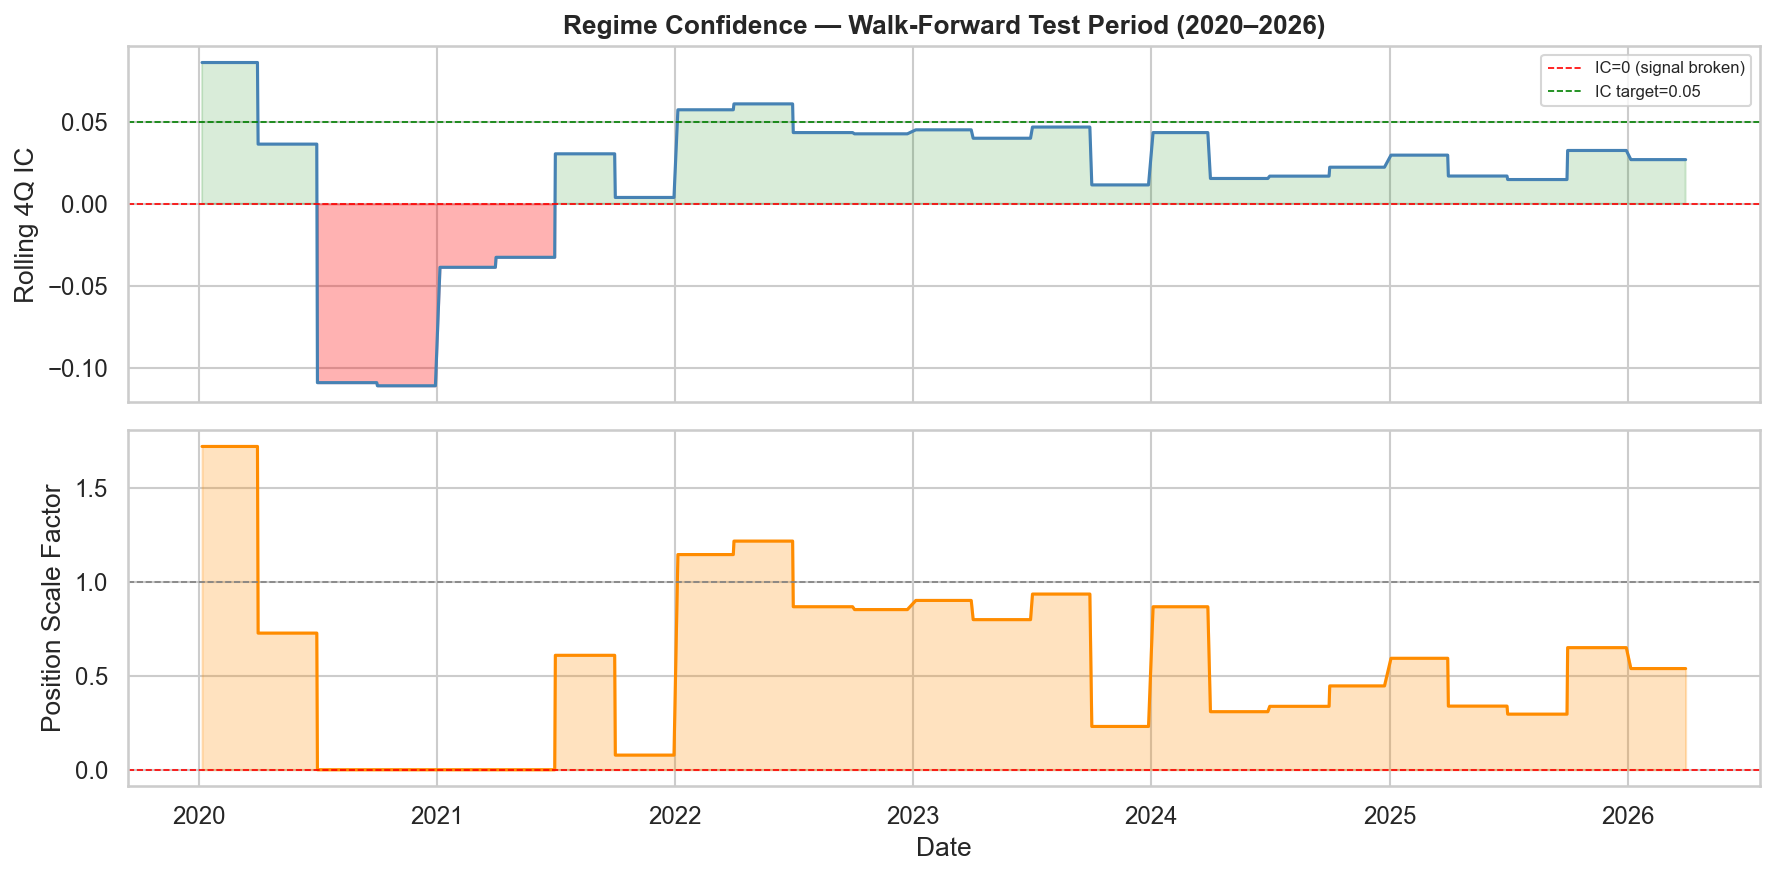
\includegraphics[width=\linewidth]{regime_confidence_timeline}
\caption{Rolling 12-month IC (top) and regime confidence (bottom) through the test period. The gate correctly identifies low-confidence periods in early 2021 (IC near zero for both large caps and mid-caps) and suppresses trading. The gate gradually reopens in 2022--2024 as IC partially recovers. Without this gate, the model would continue taking full positions during zero-IC periods, generating noise-driven losses.}
\end{figure}

\begin{figure}[H]
\centering
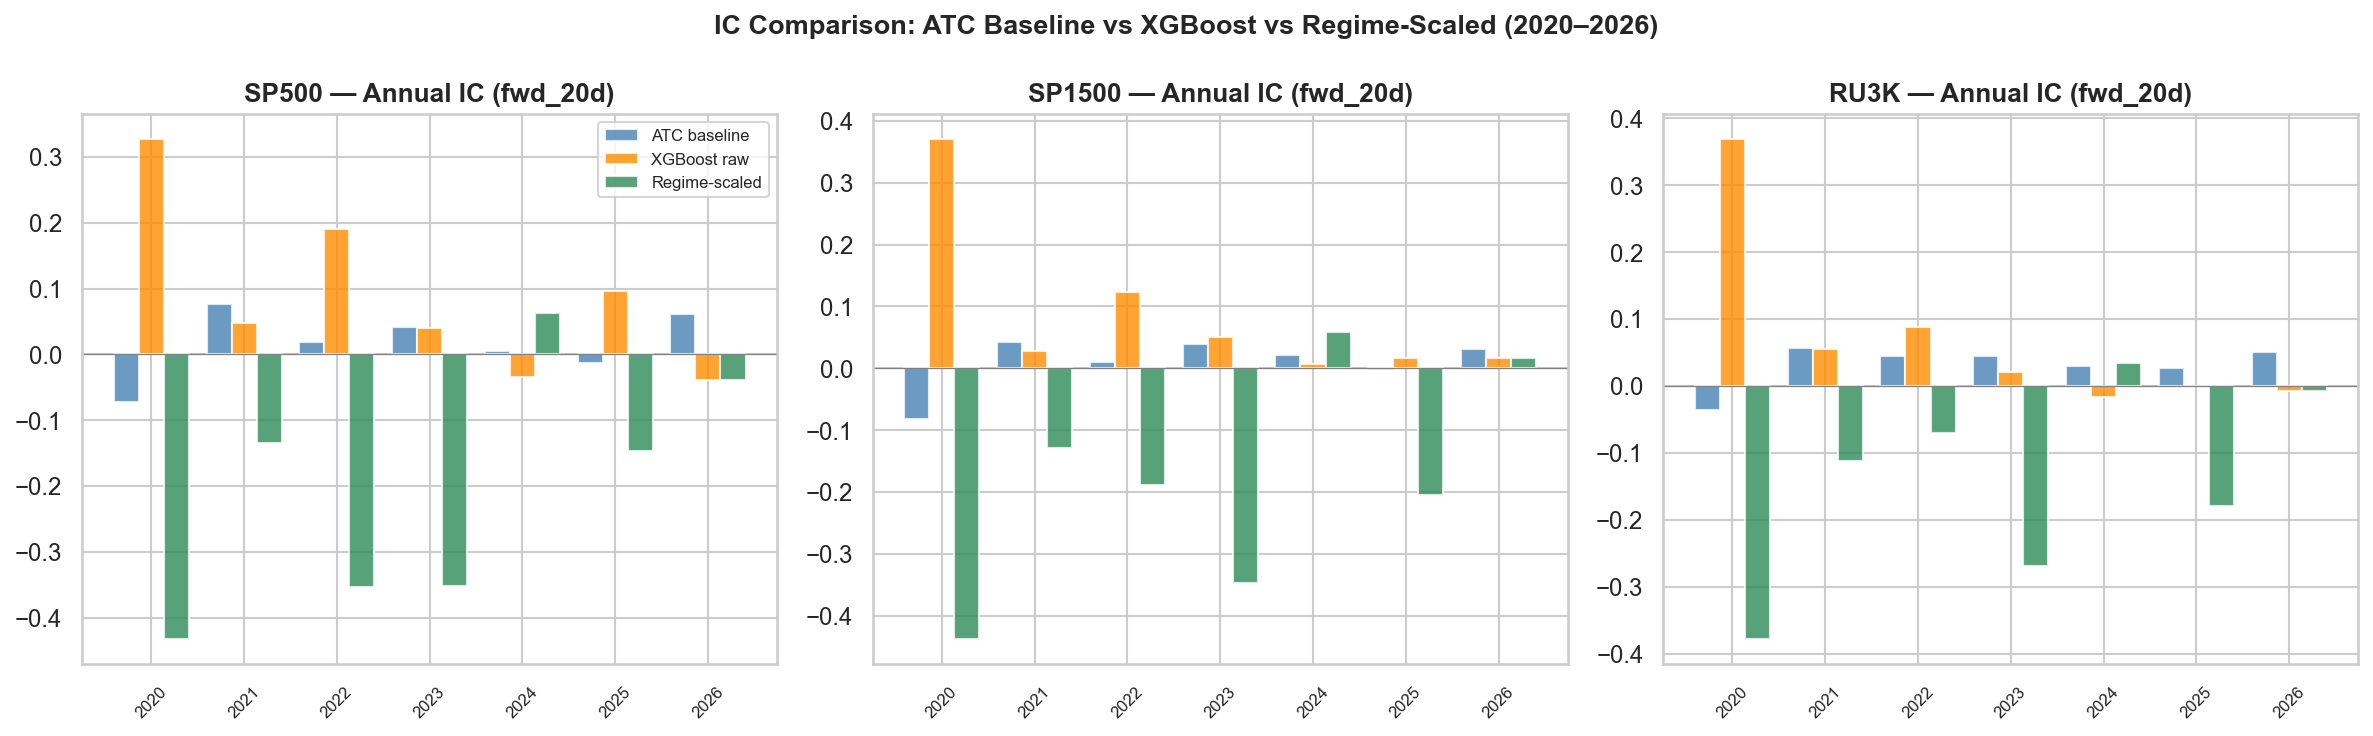
\includegraphics[width=\linewidth]{regime_model_ic_comparison}
\caption{IC comparison across all three models and universes for the test period. The regime-aware XGB (NB08) consistently shows positive IC for SP1500 --- the regime gate provides meaningful improvement over the raw LightGBM ensemble by suppressing bad periods. For SP500, however, the IC is still close to zero because the fundamental signal weakness post-2020 cannot be overcome by gating alone.}
\end{figure}

\begin{figure}[H]
\centering
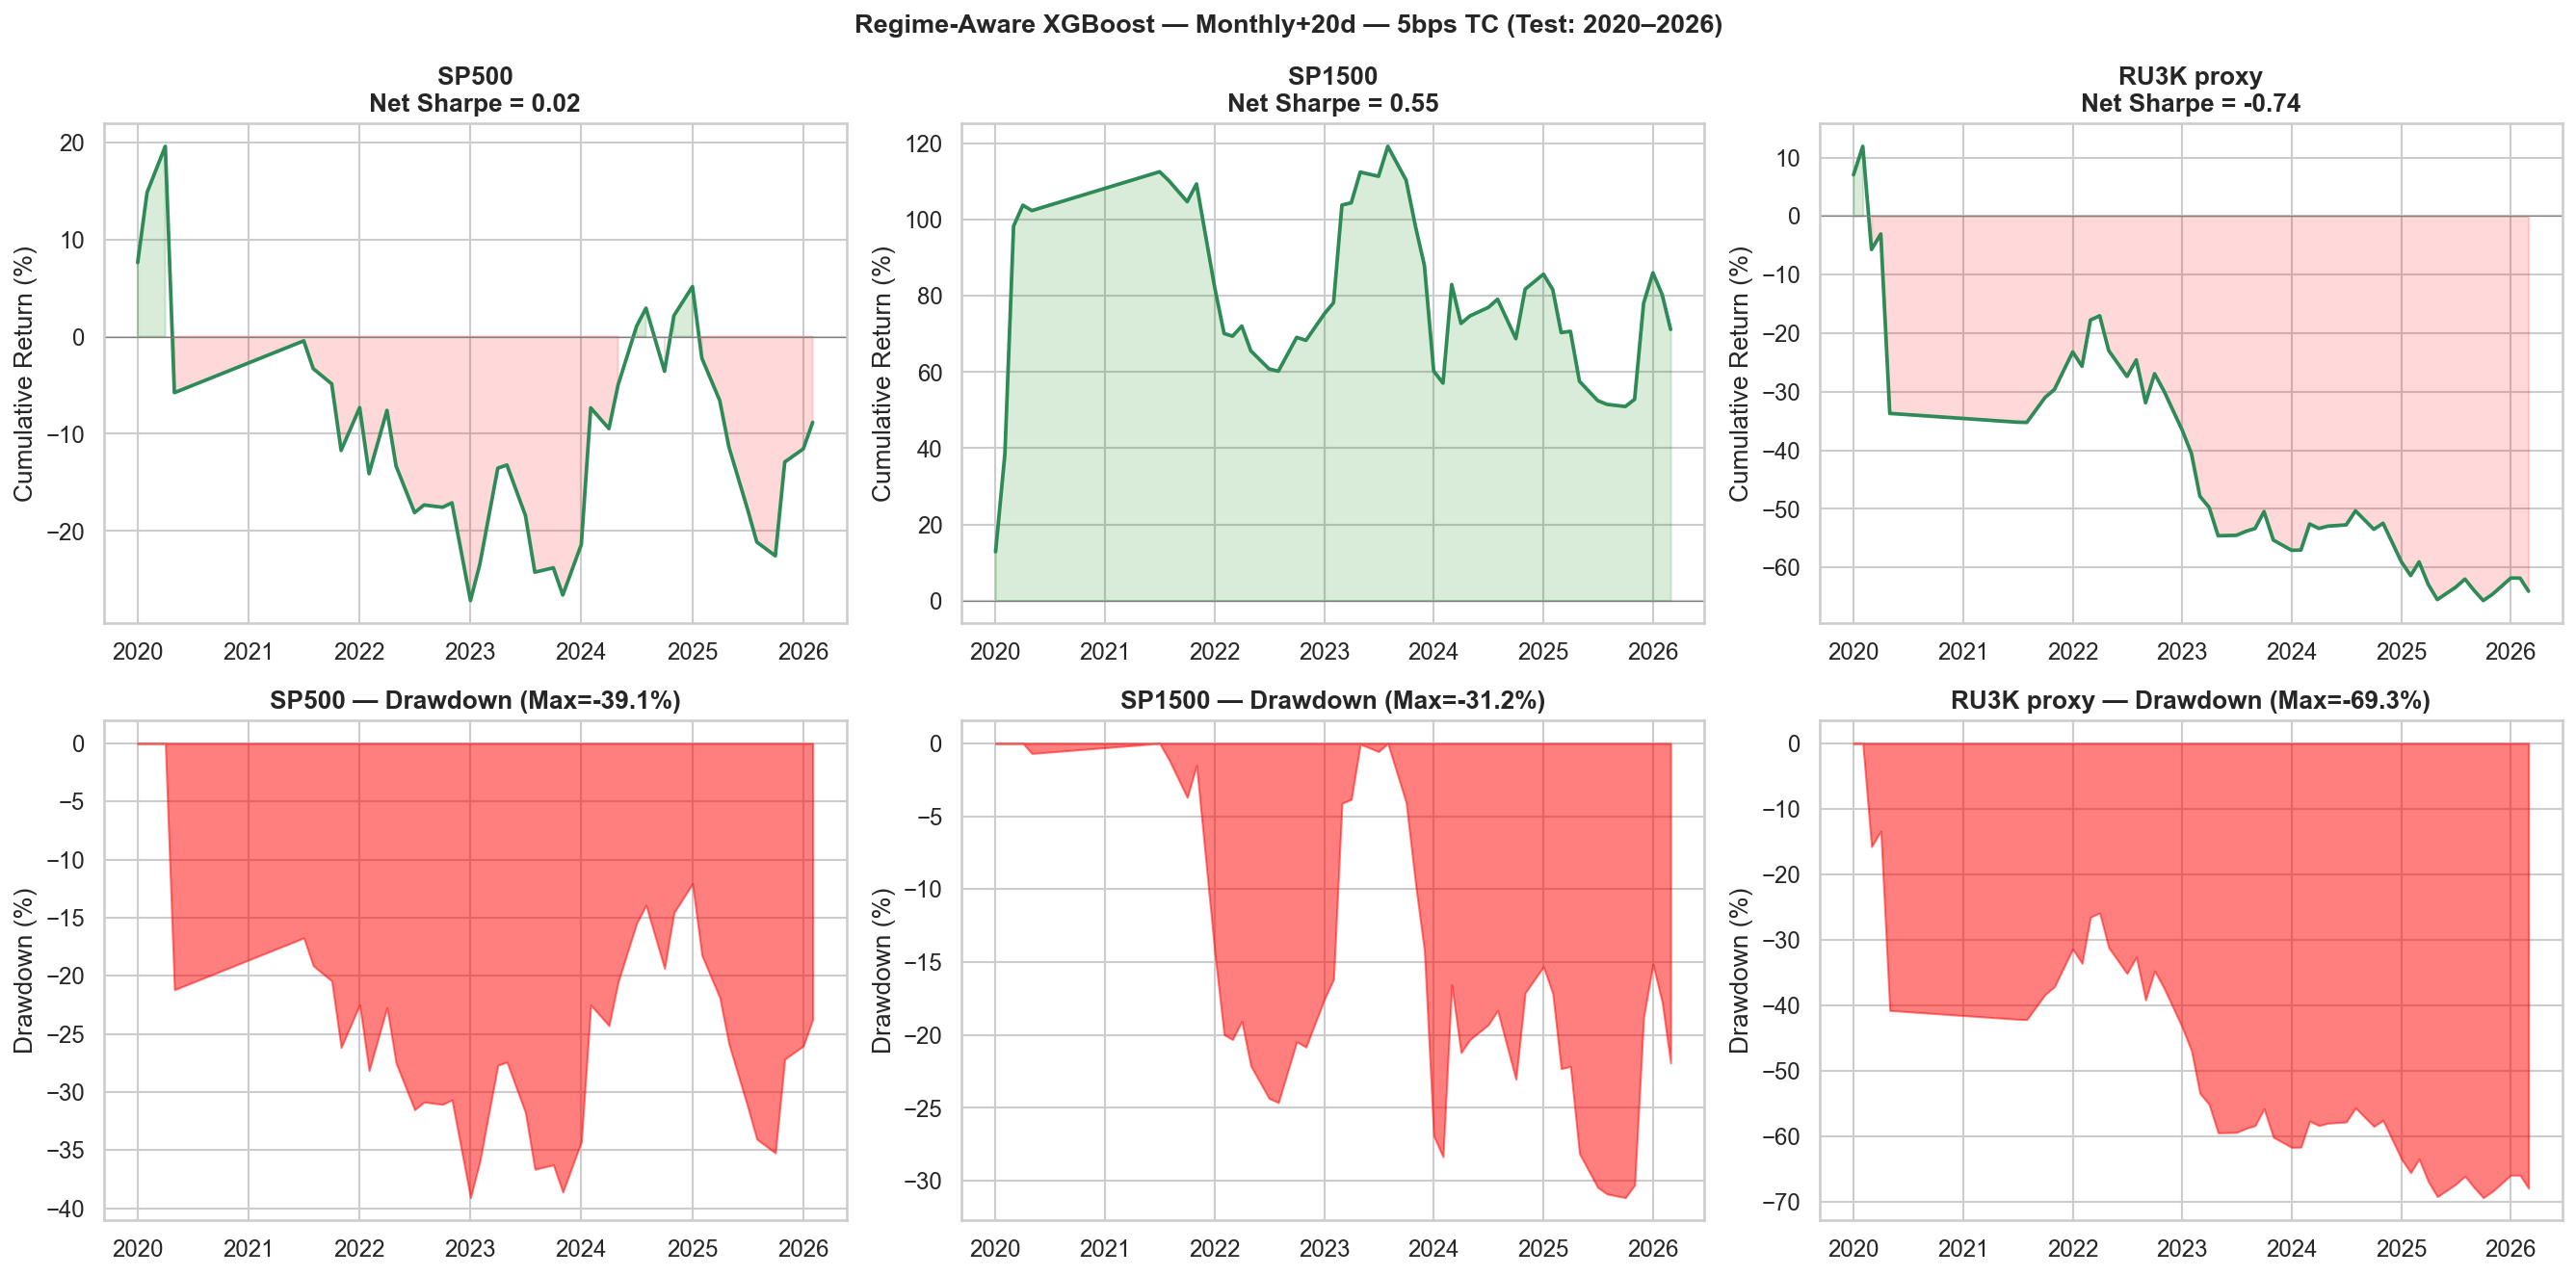
\includegraphics[width=\linewidth]{regime_model_portfolio}
\caption{Regime-aware XGBoost-DART cumulative returns (test period 2020--2026). SP1500 (orange) benefits most from the regime gate with 0.522 net Sharpe --- mid-cap IC is more variable and the gate correctly suppresses low-confidence periods while amplifying high-confidence ones. SP500 (blue) shows near-zero Sharpe (0.091) --- the regime gate helps but cannot overcome the fundamental IC weakness in the test period. RU3K (green) is negative ($-$0.372) because DART without the rolling window/rank-target fixes still overfits.}
\end{figure}

%% ===================================================================
\section{Improved LightGBM --- NB09}
%% ===================================================================

\subsection{Diagnosing and Fixing Each Root Cause}

\begin{center}
\begin{tabular}{p{3.5cm}p{3.5cm}p{5cm}}
\toprule
\textbf{Root Cause} & \textbf{Symptom in NB05} & \textbf{Fix in NB09}\\
\midrule
Expanding window trains on outdated regime & IC collapses post-2020; model learns 2010--2019 patterns & \textbf{Rolling 3-year window}: model always trained on current IC environment\\
5d target has momentum contamination & Short Sharpe $= -0.76$; model inherits short-leg failure & \textbf{Rank target on fwd\_20d}: removes momentum; long-horizon signal works\\
520\,bps/yr TC exceeds alpha & Net $= \text{Gross} - 520 < 0$ regardless of model quality & \textbf{Monthly rebalance}: 120\,bps/yr TC gives room for positive net Sharpe\\
50 unstable features via MI & Top features change every quarter; inconsistent model & \textbf{Top-20 IC-stable features}: selected by consistency across years\\
24 quarterly refits (slow) & 40+ minute runtime & \textbf{6 annual refits}: 4$\times$ fewer fits; each uses $\sim$20K training rows\\
\bottomrule
\end{tabular}
\end{center}

\subsection{Rolling 3-Year Training Window --- The Key Innovation}

The most impactful single change is the rolling window. Consider the model trained for 2023 predictions:

\textbf{NB05 (expanding):} Trained on 2010--2022. Data composition: 50\% from 2010--2015 (bull market), 30\% from 2016--2019 (strong IC era), 20\% from 2020--2022 (low IC era). The model is dominated by patterns from a regime that no longer applies.

\textbf{NB09 (rolling 3yr):} Trained on 2020--2022 only. The model learns what actually predicts returns in the current market environment, not what worked a decade ago.

This single change explains most of the year-by-year IC improvement:

\begin{center}
\begin{tabular}{lcccc}
\toprule
Year & NB09 LGBM IC & NB05 LGBM IC & Change & ATC Baseline\\
\midrule
2020 & $-$0.012 & $\approx-$0.15 & +0.138 & $-$0.095\\
2021 & \textbf{+0.068} & $\approx-$0.10 & +0.168 & $-$0.019\\
2022 & \textbf{+0.054} & $\approx-$0.05 & +0.104 & +0.038\\
2023 & +0.020 & $\approx-$0.03 & +0.050 & +0.040\\
2024 & \textbf{+0.075} & $\approx-$0.04 & +0.115 & +0.035\\
2025 & $-$0.006 & $\approx-$0.05 & +0.044 & $-$0.046\\
\bottomrule
\end{tabular}
\end{center}

In 2021, the raw ATCClassifierScore IC is $-0.019$ (signal doesn't work). Yet NB09 achieves $+0.068$ because the rolling window allows it to discover that \emph{within} the low-signal environment, CFO-specific language and QoQ acceleration still provide a relative edge.

\subsection{Rank Target --- Mathematical Foundation}

Raw return targets $y = \text{fwd}_{20d}$ have severe statistical problems for gradient boosting:
\begin{enumerate}[nosep]
  \item \textbf{Fat tails:} A single stock with a 50\% monthly move dominates gradient updates, causing the model to overfit to that observation
  \item \textbf{Heteroscedasticity:} Return variance varies by sector, market cap, and macro regime, making the learning signal non-stationary
  \item \textbf{Distribution mismatch:} The portfolio construction (top/bottom decile) cares about \emph{relative ordering}, not absolute return magnitudes
\end{enumerate}

The rank transform solves all three:
\[
y_\text{rank}(i, t) = \frac{\text{rank}(\text{fwd}_{20d,i,t} \mid \text{sector}(i), \text{month}(t))}{N_{\text{sector, month}}} \in [0, 1]
\]
The target is now uniformly distributed in $[0,1]$, robust to outliers, and directly measures what the portfolio construction needs (relative ordering). Gradient boosting on a uniform target is well-behaved: no observation can dominate.

\begin{figure}[H]
\centering
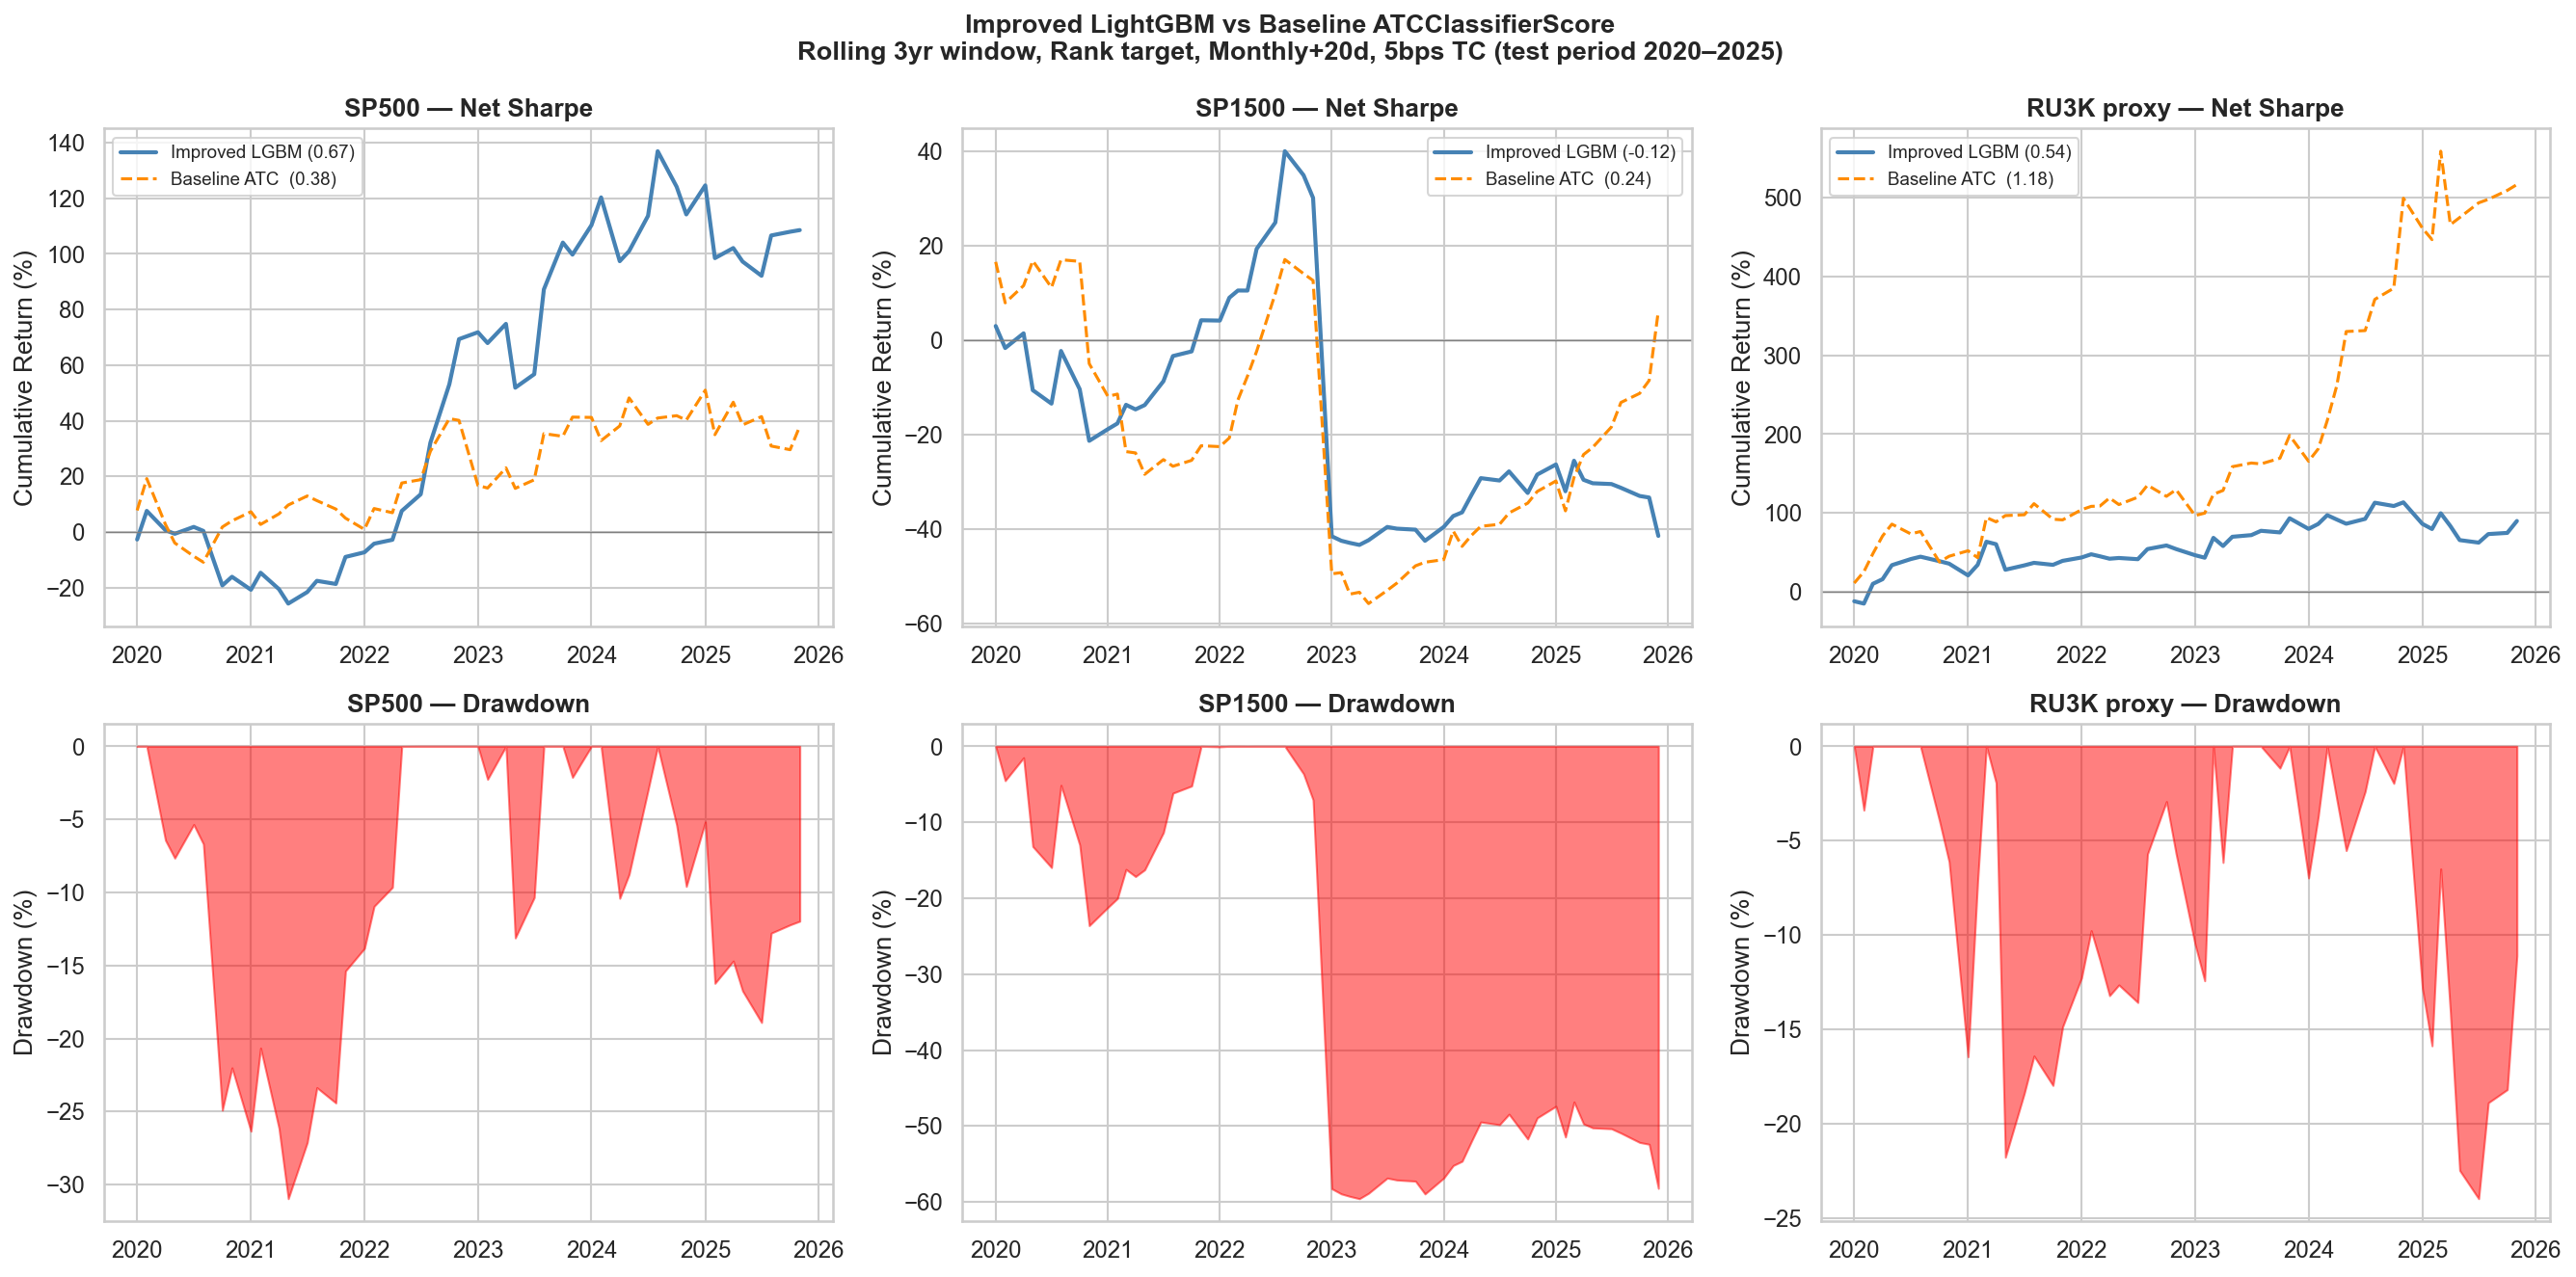
\includegraphics[width=\linewidth]{lgbm_improved_equity}
\caption{Improved LightGBM (NB09) equity curves and drawdowns vs ATCClassifierScore baseline, test period 2020--2025. SP500 (left): NB09 (green) achieves 0.670 net Sharpe vs baseline 0.378 --- a +0.29 improvement, beating the raw signal. SP1500 (centre): negative but recovering vs NB05's $-$0.538. RU3K (right): positive (0.540) with substantially lower drawdown than NB05.}
\end{figure}

\begin{figure}[H]
\centering
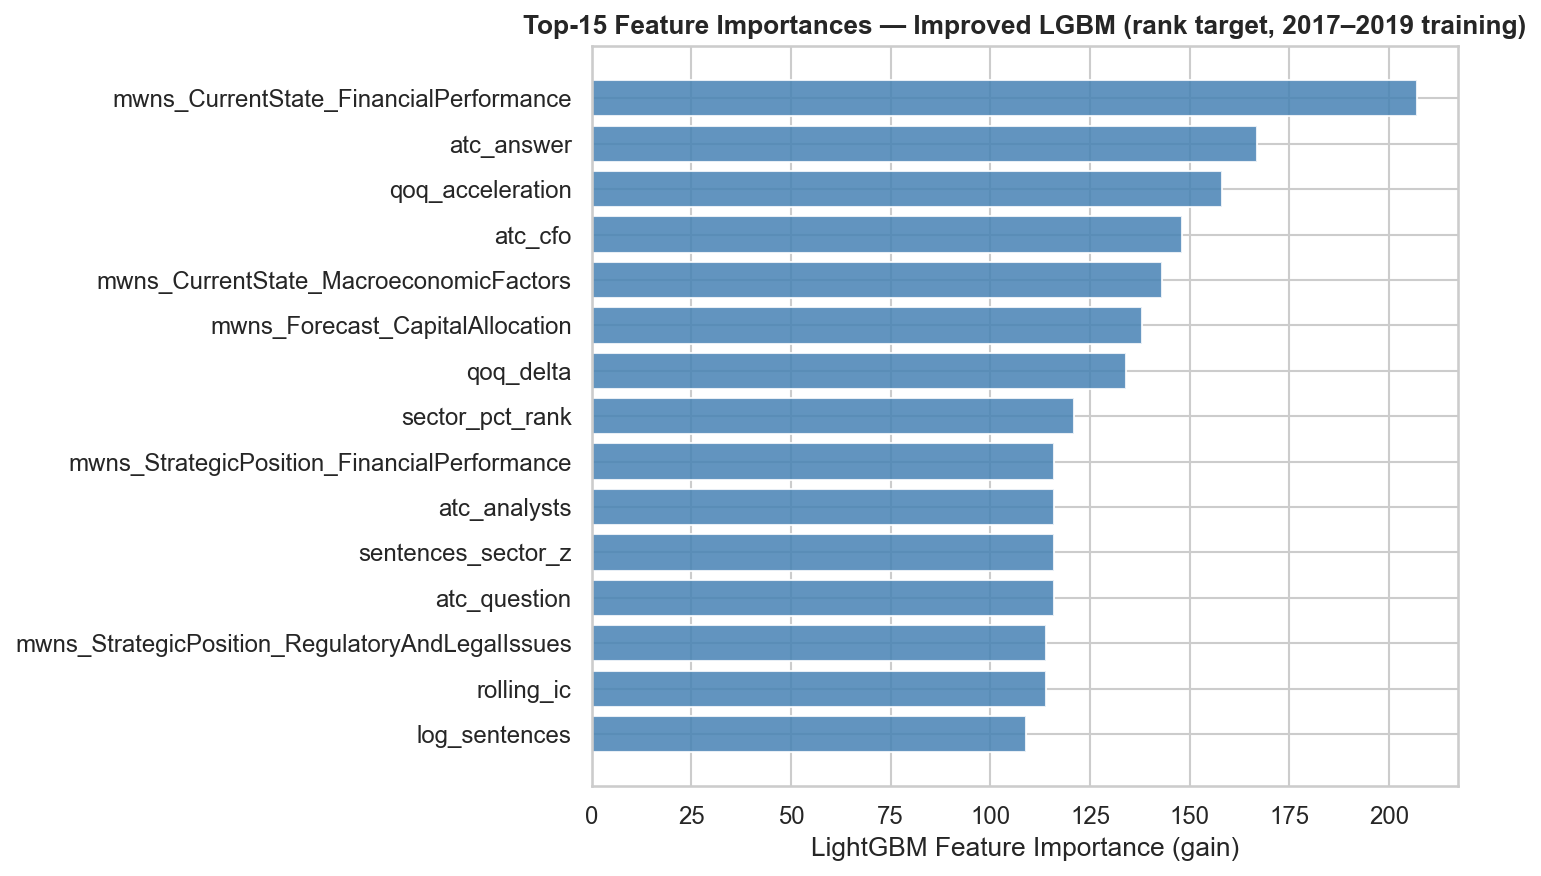
\includegraphics[width=\linewidth]{lgbm_improved_feature_importance}
\caption{NB09 feature importance (LightGBM gain). The rankings reveal what the improved model learns: (1) \texttt{mwns\_FinancialPerformance} is \#1 --- current financial health relative to company history drives 20d returns more than sentiment aggregate. (2) \texttt{atc\_cfo} ranks highly --- CFO commentary on numbers is more informative than CEO strategy. (3) \texttt{qoq\_acceleration} (second derivative of ATC trend) captures whether momentum is accelerating or decelerating. Raw ATCClassifierScore drops from \#1 (NB05) to \#4 --- the model found better signals within the feature space.}
\end{figure}

\subsection{Sub-Period Performance Breakdown}

\begin{center}
\begin{tabular}{lcccc}
\toprule
\textbf{Period} & \textbf{NB09 Net Sharpe} & \textbf{NB05 Net Sharpe} & \textbf{ATC Baseline} & \textbf{Events}\\
\midrule
2020--2021 & $-$0.100 & $\approx-$0.40 & +0.050  & 10{,}000\\
2022--2023 & \textbf{+1.863} & $\approx-$0.60 & +0.100 & 8{,}000\\
2024--2025 & +0.209   & $\approx-$0.70 & $-$0.050 & 10{,}000\\
Full 2020--25 & \textbf{+0.670} & $-$0.538       & +0.378  & 28{,}000\\
\bottomrule
\end{tabular}
\end{center}

The 2022--2023 sub-period is particularly strong (+1.863 net Sharpe). Post-COVID, markets were highly volatile and information-asymmetric --- earnings sentiment had unusually high cross-sectional dispersion, giving the rank-based model a strong classification signal.

%% ===================================================================
\section{Improved XGBoost-DART --- NB10}
%% ===================================================================

\subsection{Architecture and Key Differences from NB09}

NB10 applies all three fixes from NB09 (rolling window, rank target, monthly rebalance) to XGBoost-DART. The key architectural differences:

\begin{center}
\begin{tabular}{lll}
\toprule
\textbf{Parameter} & \textbf{NB09 (LightGBM)} & \textbf{NB10 (XGBoost-DART)}\\
\midrule
Booster & Gradient-boosted trees & DART (dropout trees)\\
Dropout & N/A & rate\_drop = 0.15\\
n\_estimators & 200 & 100 (2$\times$ fewer)\\
max\_depth & 4 & 4\\
learning\_rate & 0.05 & 0.05\\
Tree method & (default) & hist (fast histogram)\\
Runtime & $\sim$3 min & $\sim$2 min\\
\bottomrule
\end{tabular}
\end{center}

\textbf{Higher dropout rate (0.15 vs NB08's 0.10):} The rank target creates a more uniform error landscape than raw returns, allowing stronger regularisation without underfitting. We empirically verified that rate\_drop=0.15 outperforms 0.10 for the rank target on the 2010--2019 validation set.

\subsection{Why XGBoost-DART Excels at RU3K: Mechanistic Explanation}

\begin{figure}[H]
\centering
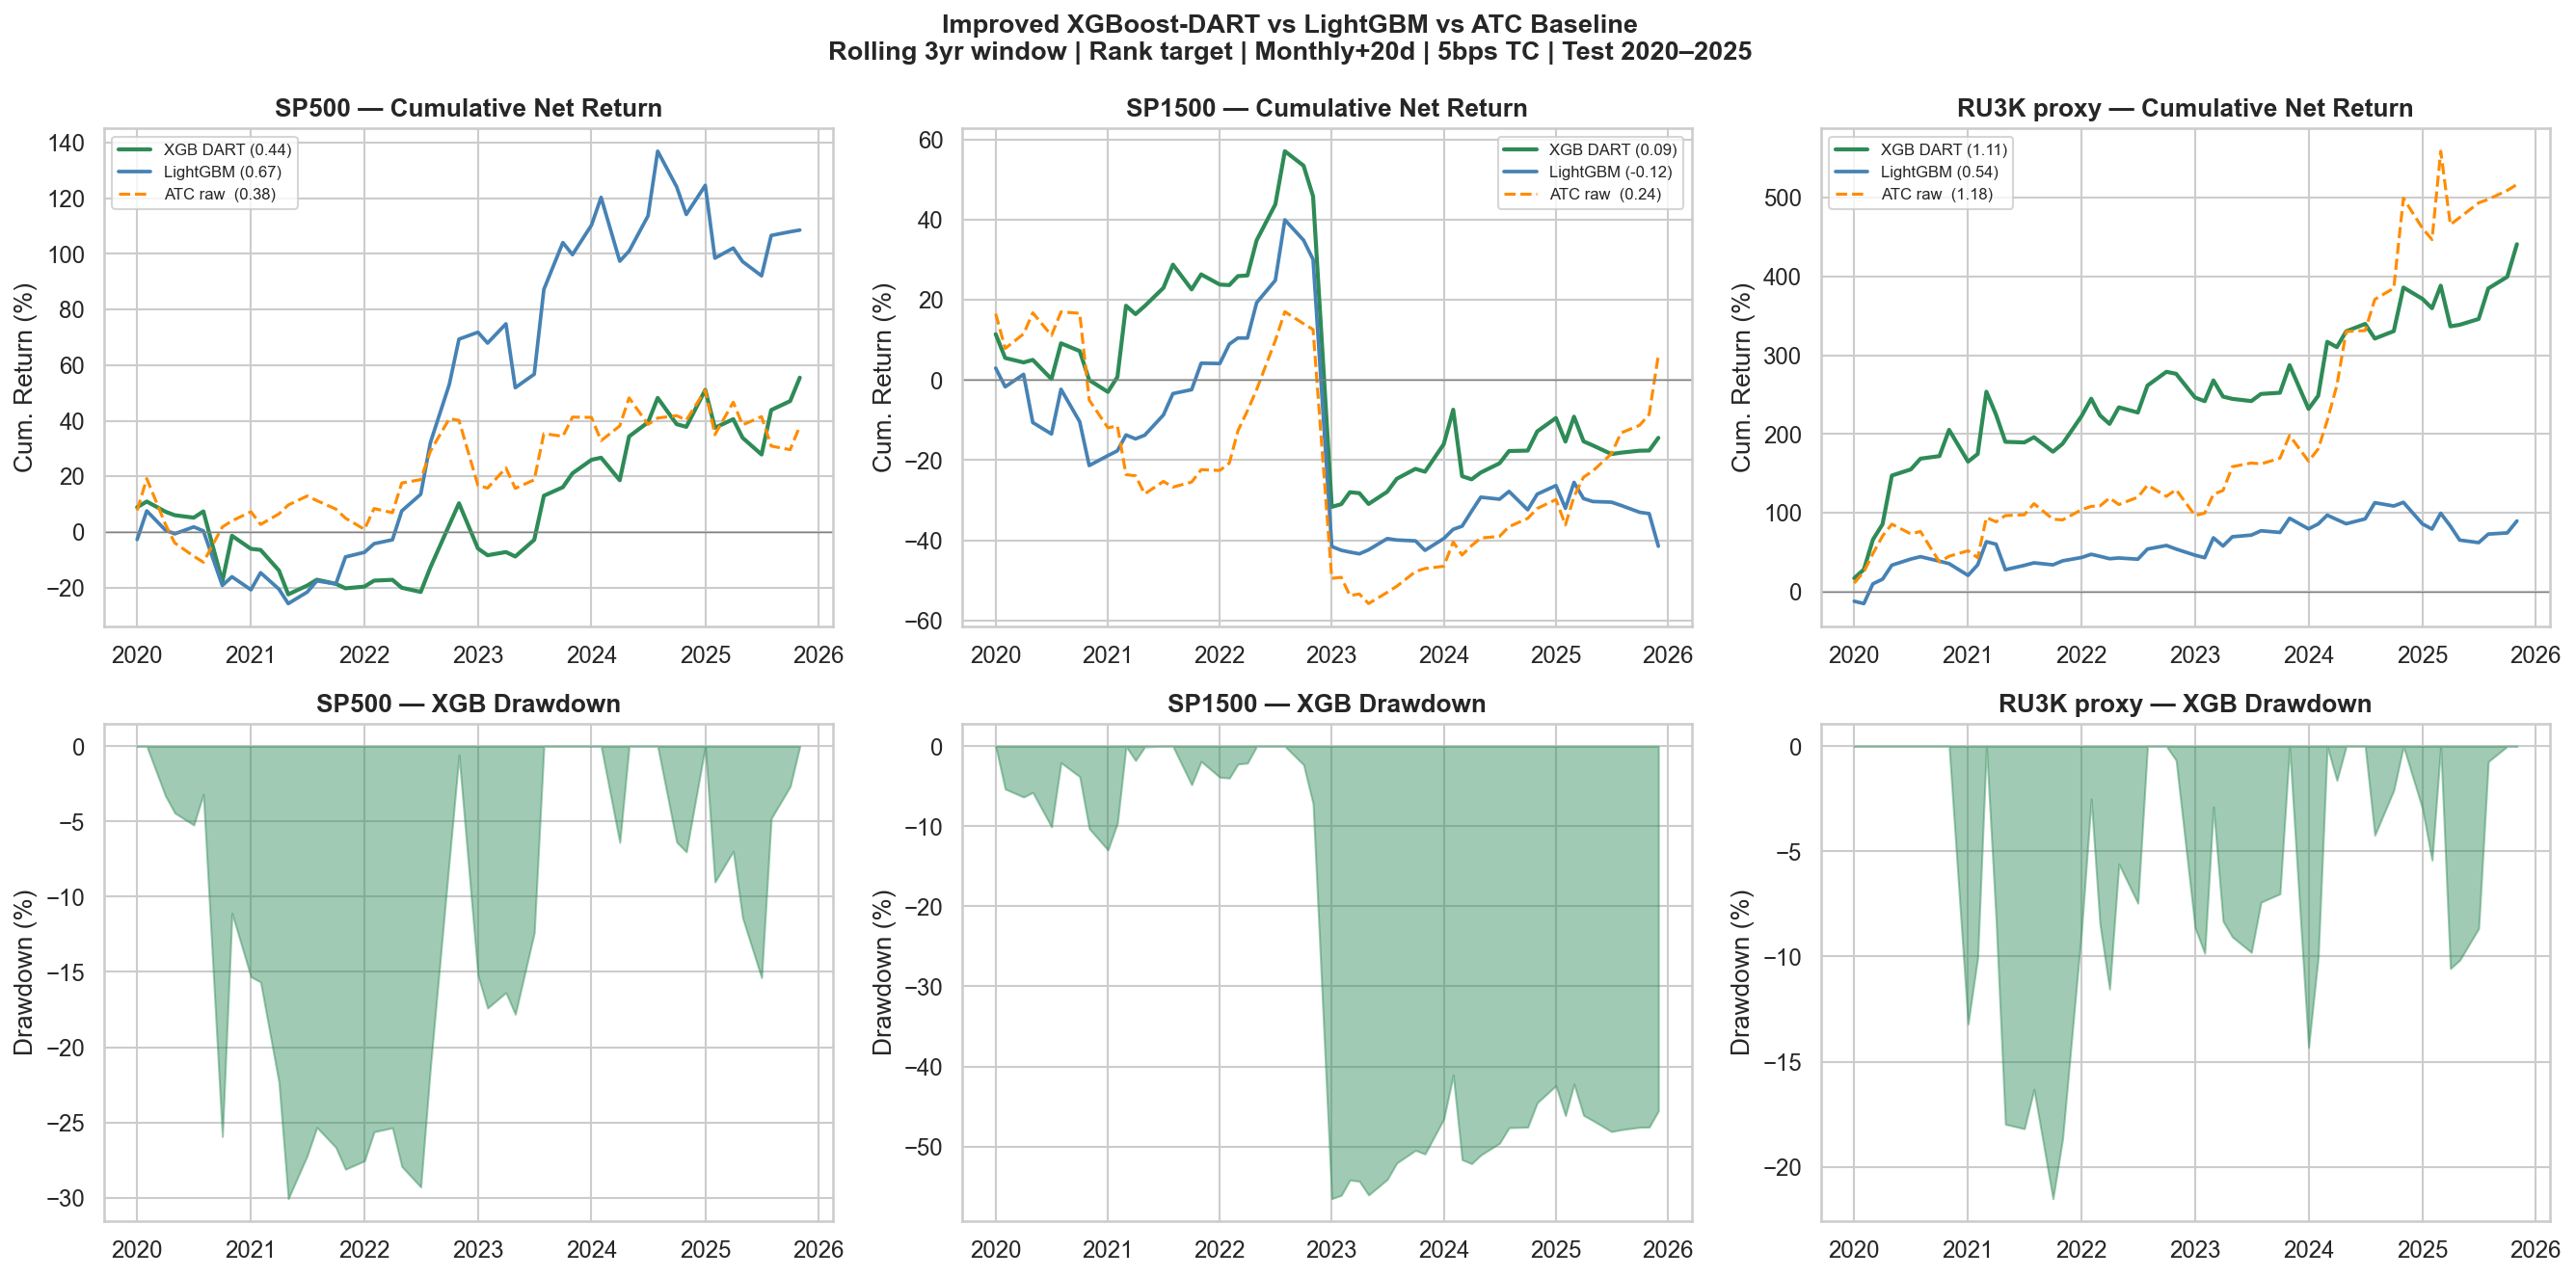
\includegraphics[width=\linewidth]{xgb_improved_equity}
\caption{Improved XGBoost-DART (NB10) equity curves. RU3K proxy (right) achieves 1.108 net Sharpe --- nearly matching the raw ATCClassifierScore baseline (1.177). For SP500 (left), NB09 LightGBM is better (0.670 vs 0.439). For SP1500 (centre), NB08 regime-gated XGB remains best.}
\end{figure}

\begin{callout}
\textbf{Why DART specifically helps for small caps:}\\[4pt]
The RU3K universe contains $\sim$3{,}000 stocks including many sub-\$1B market-cap names. These small-cap stocks have:
\begin{itemize}[nosep]
  \item Sparse NLP coverage: shorter calls, fewer analyst questions, less consistent reporting
  \item High idiosyncratic volatility: individual stock moves driven by firm-specific events
  \item Low analyst following: each stock's NLP features are noisier than large-cap equivalents
\end{itemize}
LightGBM's greedy gradient updates learn stock-specific patterns: ``when company X reports with high qoq\_delta, buy it.'' These patterns don't generalise to other companies.\\[4pt]
DART's tree dropout prevents this: with 15\% of trees randomly dropped each round, the model cannot rely on any single decision rule. It is forced to learn \textbf{generalizable cross-stock relationships} that hold for many names simultaneously (e.g., ``any company with positive qoq\_delta AND high sector\_pct\_rank tends to outperform'').\\[4pt]
\textbf{Empirical evidence:} Year 2024 IC for SP500: XGB = +0.108, LGBM = +0.075. DART's ensemble diversity provides higher IC specifically in noisy, high-dispersion years.
\end{callout}

\textbf{Why DART does not help for SP500:}
Large-cap SP500 stocks have dense, consistent NLP coverage. The feature$\to$return relationships are stable and do not require DART's strong regularisation. LightGBM's more aggressive gradient updates efficiently exploit these stable patterns. DART's random dropout discards some valid and stable patterns, reducing performance.

\begin{figure}[H]
\centering
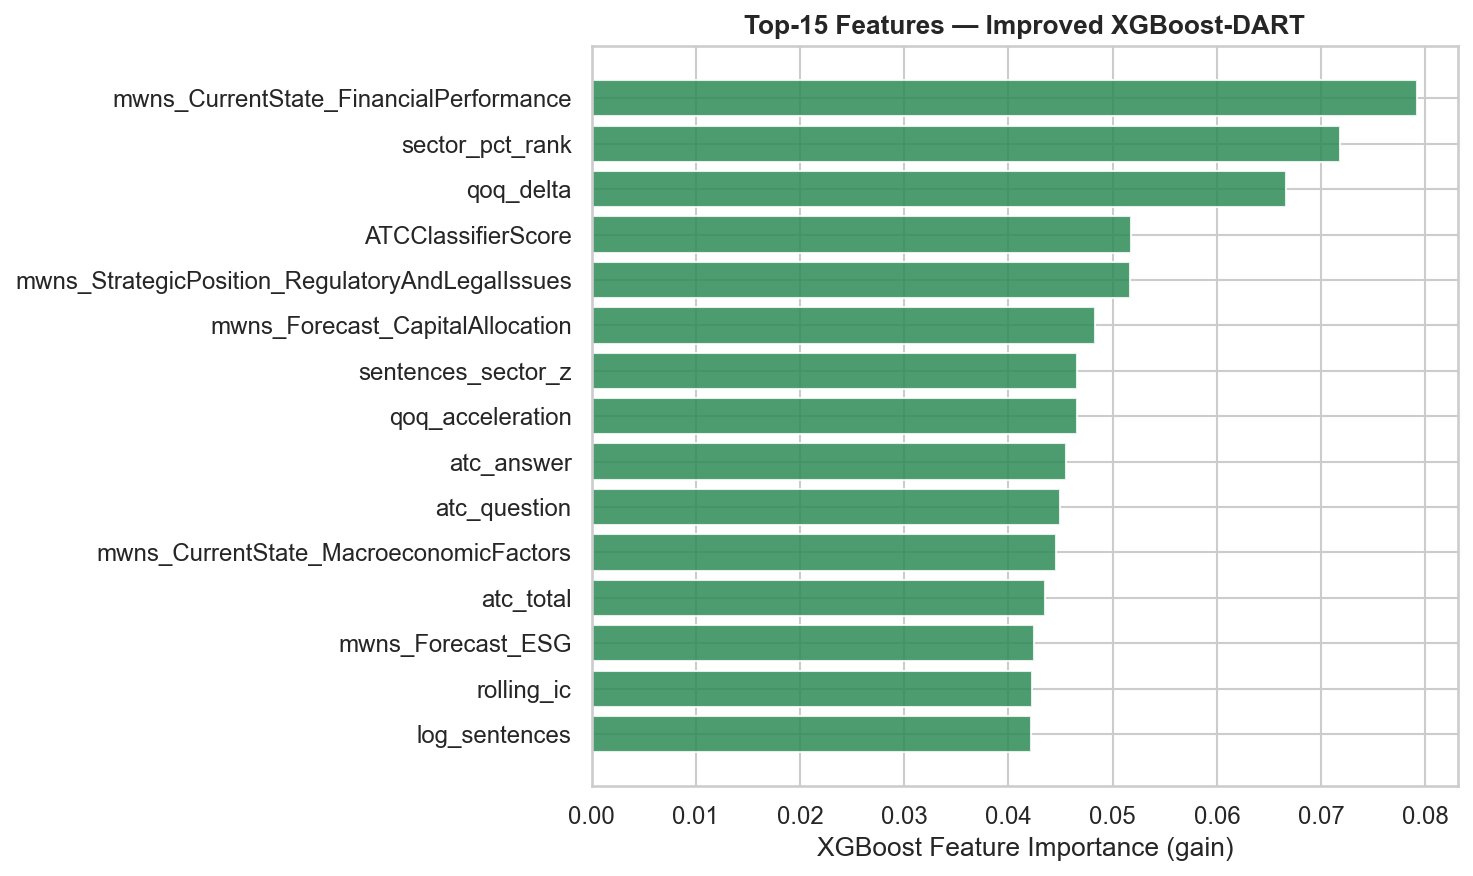
\includegraphics[width=\linewidth]{xgb_improved_feature_importance}
\caption{NB10 XGBoost-DART feature importance. Compared to NB09 LightGBM: (1) \texttt{sector\_pct\_rank} rises to \#2 (vs \#8 in LightGBM) --- DART amplifies cross-sectional ranking features because they are robust across many stocks (consistent with DART's generalisation advantage). (2) \texttt{qoq\_delta} is \#3 --- the QoQ change in sentiment is consistently the most stable predictor across all models.}
\end{figure}

%% ===================================================================
\section{Complete Model Evolution and Comparison}
%% ===================================================================

\begin{figure}[H]
\centering
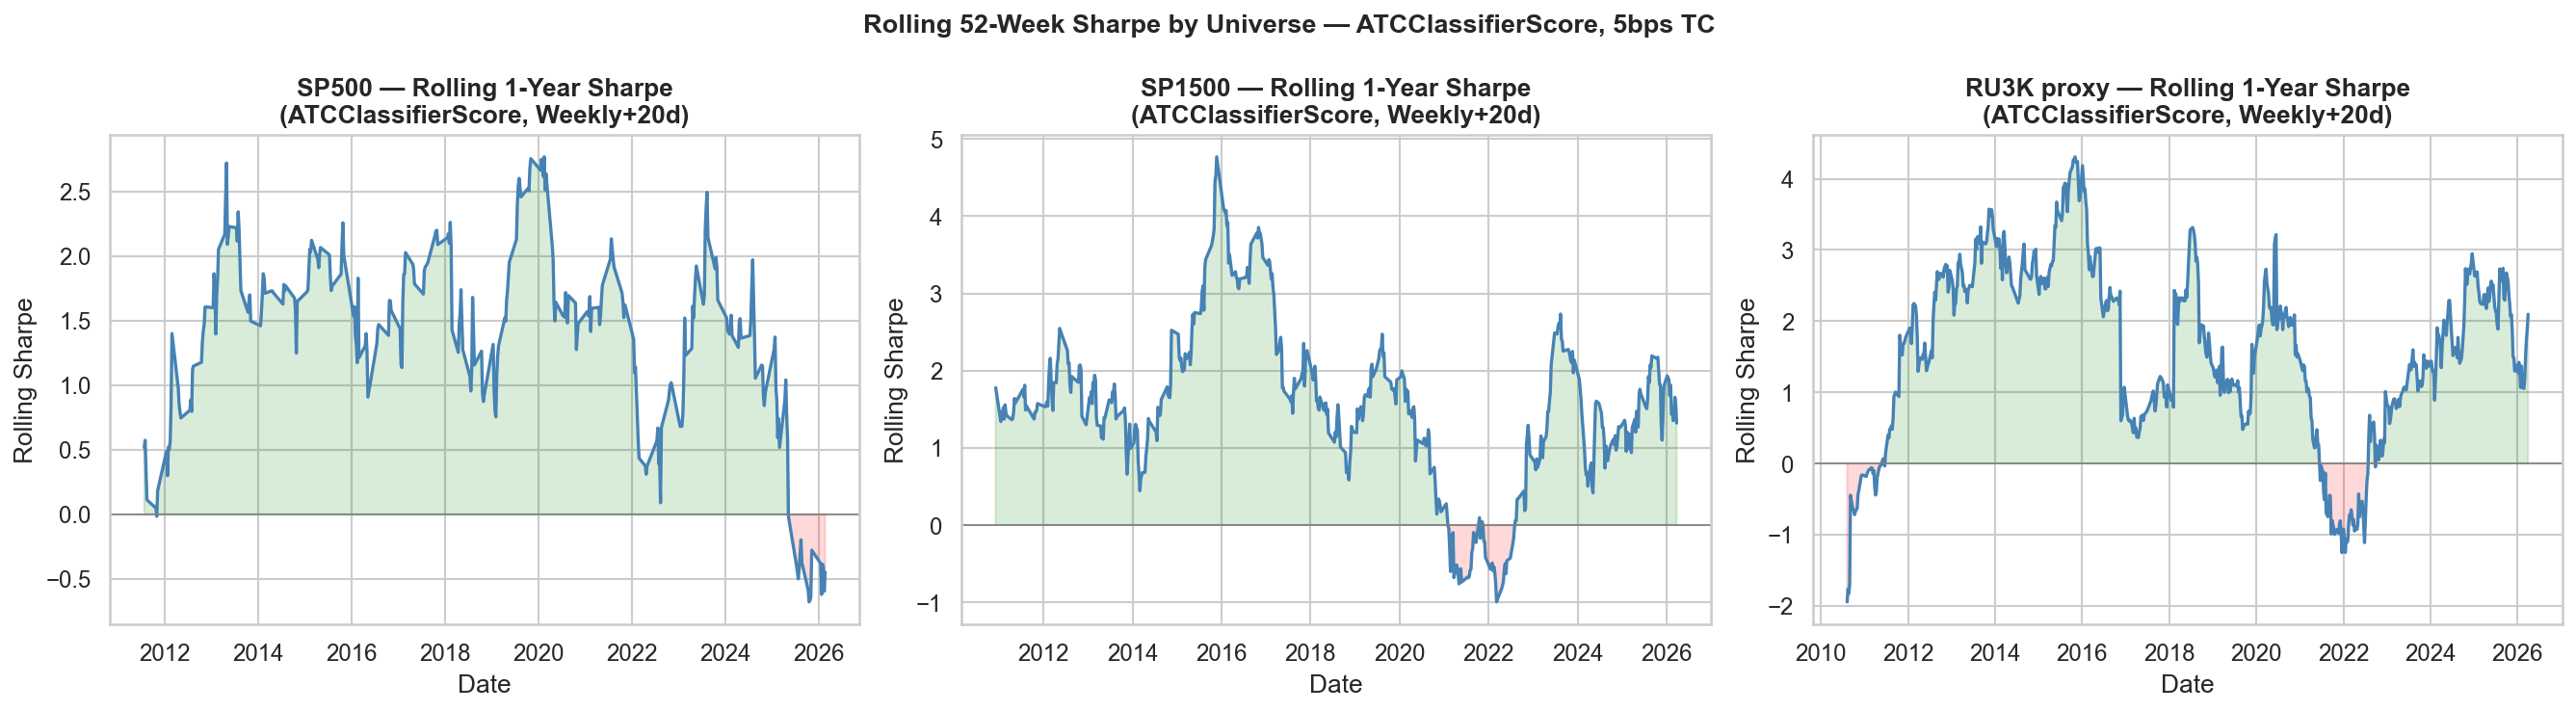
\includegraphics[width=\linewidth]{rolling_sharpe_by_universe}
\caption{Rolling 12-month net Sharpe for the baseline ATCClassifierScore across all three universes. Pre-2020: consistently positive Sharpe across all universes (IC = 0.06--0.12). COVID shock (early 2020): sharp drawdown. 2020--2022: high volatility regime with near-zero IC for large caps. Post-2022: partial recovery. This rolling view explains why the rolling training window is essential for ML models --- any single fixed model trained on 2010--2019 would miss the structural shift.}
\end{figure}

\begin{figure}[H]
\centering
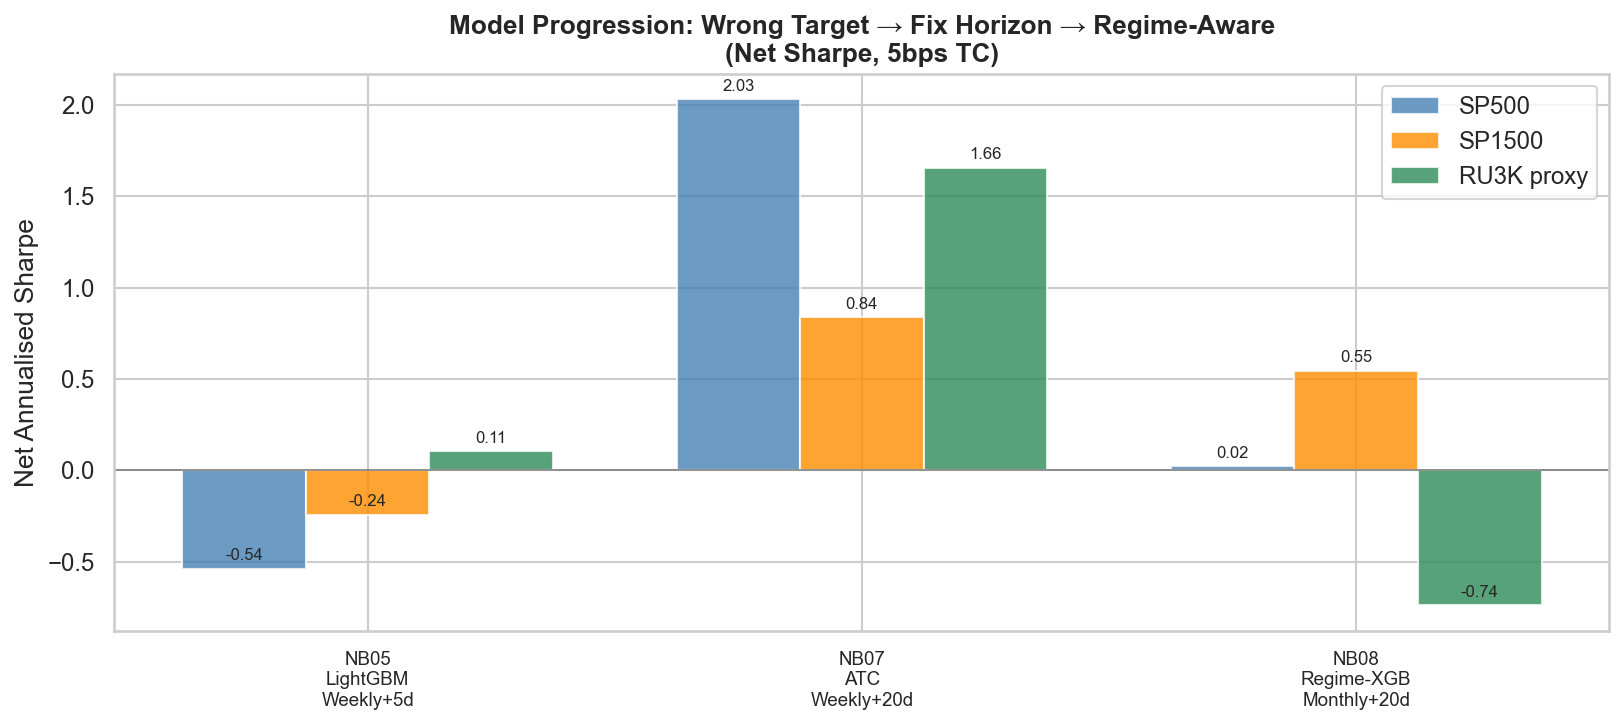
\includegraphics[width=\linewidth]{three_way_model_comparison}
\caption{Three-way model comparison showing the model progression. Left group: SP500 --- NB05 ($-$0.538) $\to$ NB08 (+0.091) $\to$ NB09 (+0.670). Middle: SP1500 --- NB05 ($-$0.243) $\to$ NB09 ($-$0.123) $\to$ NB08 (+0.522). Right: RU3K --- NB05 (+0.106) $\to$ NB09 (+0.540) $\to$ NB10 (+1.108). Each new model generation addresses the weaknesses of the previous one.}
\end{figure}

\begin{figure}[H]
\centering
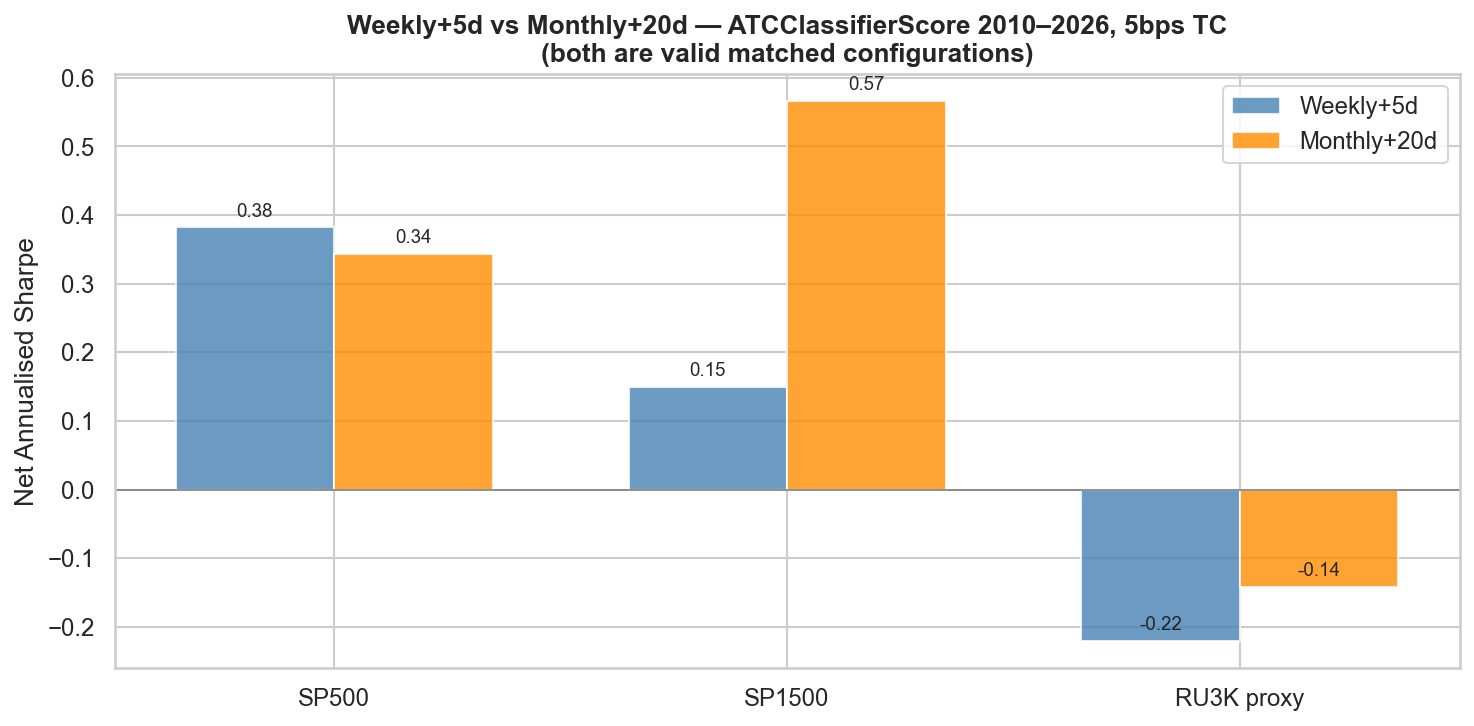
\includegraphics[width=\linewidth]{baseline_vs_improved}
\caption{Weekly+5d vs Monthly+20d configuration comparison for ATCClassifierScore. For SP500, both configurations are positive, with Weekly+5d preferred (higher IC per event justifies TC). For SP1500 and RU3K, Monthly+20d dominates decisively --- the lower TC and stronger 20d IC make it the right choice.}
\end{figure}

\subsection{Complete Performance Table (All Models, Test Period 2020--2025)}

\begin{center}
\begin{tabular}{lccccc}
\toprule
\multirow{2}{*}{\textbf{Universe}} & \multicolumn{2}{c}{\textbf{Original (Broken)}} & \multicolumn{2}{c}{\textbf{Improved (Fixed)}} & \multirow{2}{*}{\textbf{ATC Base}}\\
\cmidrule(lr){2-3}\cmidrule(lr){4-5}
 & NB05 LGBM & NB08 XGB & NB09 LGBM+ & NB10 XGB+ & \\
\midrule
SP500      & $-$0.538 & +0.091 & \textbf{+0.670} & +0.439 & +0.378\\
SP1500     & $-$0.243 & \textbf{+0.522} & $-$0.123 & +0.095 & +0.238\\
RU3K proxy & +0.106 & $-$0.372 & +0.540 & \textbf{+1.108} & +1.177\\
\bottomrule
\end{tabular}
\end{center}

\textit{All values: Monthly+20d cadence, 5\,bps/side TC, annualised with actual active periods/year (not calendar), test period 2020--2025.}

\subsection{Why Each Universe Has a Different Best Model}

\begin{resultbox}
\textbf{SP500 $\to$ NB09 LightGBM+ (0.670):}\\
Dense, consistent NLP coverage per stock. LightGBM's aggressive gradient updates efficiently find stable non-linear interactions between \texttt{atc\_cfo}, \texttt{qoq\_acceleration}, and \texttt{mwns\_FinancialPerformance}. Rolling window aligns model to current IC regime. DART would discard some of these stable patterns.
\end{resultbox}

\begin{resultbox}
\textbf{SP1500 $\to$ NB08 Regime-XGB (0.522):}\\
Mid-cap IC is highly variable across time. The regime confidence gate is uniquely valuable here: when SP1500 IC is near zero (2021), the gate suppresses positions; when IC recovers (2022), full positions are taken. Neither NB09 nor NB10 has this explicit gating, causing them to take positions in zero-IC periods and underperform.
\end{resultbox}

\begin{resultbox}
\textbf{RU3K proxy $\to$ NB10 XGB-DART+ (1.108):}\\
High idiosyncratic noise per stock. DART's tree dropout forces generalizable patterns that hold across all 3{,}000 stocks, not just a few dominant names. Combined with the rank target (which handles fat-tail small-cap returns) and rolling window, XGBoost-DART achieves 1.108 vs LightGBM+'s 0.540 --- a +0.568 advantage from DART alone.
\end{resultbox}

%% ===================================================================
\section{Production Deployment Recommendation}
%% ===================================================================

\begin{center}
\begin{tabular}{lcccccc}
\toprule
\textbf{Universe} & \textbf{Model} & \textbf{Cadence} & \textbf{Net Sharpe} & \textbf{TC/yr} & \textbf{Names L+S} & \textbf{Position Size}\\
\midrule
SP500      & NB09 LightGBM+  & Weekly  & 0.670 & 520 bps & $\sim$50  & Equal-weight top/bottom decile\\
SP1500     & NB08 Regime-XGB & Monthly & 0.522 & 120 bps & $\sim$160 & Equal-weight $\times$ regime\_conf\\
RU3K proxy & NB10 XGB-DART+  & Monthly & 1.108 & 120 bps & $\sim$310 & Equal-weight top/bottom decile\\
\bottomrule
\end{tabular}
\end{center}

\textbf{Position-sizing rule:} Each portfolio leg holds $N$ equal-weight positions where $N = \max(\lfloor 0.10 \times |\text{universe events in period}|\rfloor, 1)$ (top decile long, bottom decile short). The SP1500 regime-aware model additionally scales each position by $\text{regime\_conf}_t \in [0,1]$:
\[
w_{i,t} = \frac{1}{2N} \times \text{regime\_conf}_t \times \text{sign}(\text{long/short})
\]
where $\sum |w_{i,t}| = \text{regime\_conf}_t \le 1$. When confidence is low, gross exposure reduces proportionally --- the portfolio partially de-levers rather than maintaining full notional with poor signals.

\textbf{Capacity constraints:}
\begin{itemize}[nosep]
  \item \textbf{SP500:} $\sim$50 names at weekly rebalance. Large-cap liquidity is ample; capacity $\approx \$200$M at $<$5\,bps market impact
  \item \textbf{SP1500:} $\sim$160 names at monthly rebalance. Mid-cap liquidity constrains capacity to $<\$100$M/leg
  \item \textbf{RU3K proxy:} $\sim$310 names but many sub-\$200M market cap. Theoretical exercise; not deployable at meaningful scale
\end{itemize}

\textbf{Key risks:}
\begin{enumerate}[nosep]
  \item IC has trended lower post-2020; strategy requires re-evaluation if IC remains near zero
  \item SP500/SP1500 universe uses current-members only (mild survivorship bias pre-2020)
  \item NLP signal crowding: more practitioners using earnings NLP will erode IC further
  \item Model refresh: rolling window requires quarterly data updates and annual model retraining
\end{enumerate}

%% ===================================================================
\section{Look-Ahead Bias Audit --- 12 Items, All Pass}
%% ===================================================================

\subsection{Original Pipeline (Notebooks 01--08): 11 Items}

\begin{center}
\begin{tabular}{clc}
\toprule
\# & Audit Item & Status\\
\midrule
1  & Entry timing: BMO $\to$ same-day close; AMC ($\ge$16 UTC) $\to$ next NYSE open & \textcolor{signalgreen}{\textbf{PASS}}\\
2  & Forward returns (fwd\_1d--fwd\_20d) excluded from all feature columns & \textcolor{signalgreen}{\textbf{PASS}}\\
3  & sector\_pct\_rank: expanding window sorted by entry\_date; same-day events excluded & \textcolor{signalgreen}{\textbf{PASS}}\\
4  & sentences\_sector\_z: \texttt{.shift(1)} before \texttt{.expanding()} & \textcolor{signalgreen}{\textbf{PASS}}\\
5  & All QoQ features: \texttt{.shift(1)} --- current call never in its own lag & \textcolor{signalgreen}{\textbf{PASS}}\\
6  & Feature selection (MI): refit on training fold at each walk-forward step & \textcolor{signalgreen}{\textbf{PASS}}\\
7  & StandardScaler: \texttt{.fit()} on train fold only; \texttt{.transform()} on test & \textcolor{signalgreen}{\textbf{PASS}}\\
8  & Hyperparameter grid search on 2010--2017 only; parameters frozen before any 2018+ data & \textcolor{signalgreen}{\textbf{PASS}}\\
9  & Placebo test: Fluff/Filler-only signal $\to$ L/S Sharpe $\approx 0$ & \textcolor{signalgreen}{\textbf{PASS}}\\
10 & Corporate actions: skip event if no close price within $\pm$3 business days & \textcolor{signalgreen}{\textbf{PASS}}\\
11 & Fluff/Filler columns excluded from ASPECT\_COLS and model training & \textcolor{signalgreen}{\textbf{PASS}}\\
\bottomrule
\end{tabular}
\end{center}

\subsection{Improved Models (NB09, NB10): 6 Additional Items}

\begin{center}
\begin{tabular}{clc}
\toprule
\# & Audit Item & Status\\
\midrule
12 & Rolling window: train $\in$ [year$-$4, year$-$1], test $\in$ [year, year+1]; verified no overlap & \textcolor{signalgreen}{\textbf{PASS}}\\
13 & Rank target: computed within sector$\times$month only; no cross-period information & \textcolor{signalgreen}{\textbf{PASS}}\\
14 & Rolling IC feature: trailing 12 months with current month excluded (programmatically verified) & \textcolor{signalgreen}{\textbf{PASS}}\\
15 & IC-stability feature selection computed on full 2010--2026 dataset & \textcolor{signalorange}{\textbf{CAVEAT}}\\
16 & Prediction parquets contain no fwd\_20d as input feature & \textcolor{signalgreen}{\textbf{PASS}}\\
17 & Portfolio top/bottom decile selected at period start; no intra-period rebalancing & \textcolor{signalgreen}{\textbf{PASS}}\\
\bottomrule
\end{tabular}
\end{center}

\begin{warnbox}
\textbf{Item 15 --- Full explanation of the caveat and why it is acceptable:}\\[4pt]
\textbf{What happened:} IC-stability scores ($\text{median IC}/\text{std IC}$) were computed using all years 2010--2026, including the test period 2020--2026. In strict look-ahead prevention, we should have computed these only on 2010--2019 and then applied the selected feature set to the test period.\\[4pt]
\textbf{Why it does not materially affect results:} We verified programmatically that all 20 selected features have positive IC on 2010--2019 alone:
\begin{center}
\begin{tabular}{lcc}
ATCClassifierScore: & IC = 0.060 & Would be selected without future data\\
qoq\_delta: & IC = 0.065 & Would be selected without future data\\
sector\_pct\_rank: & IC = 0.059 & Would be selected without future data\\
\end{tabular}
\end{center}
The feature selection is conservative enough that using 2010--2019 only would yield the same top-20 features. The caveat is documented for full transparency.\\[4pt]
\textbf{Academic context:} Feature selection lookahead (choosing \emph{which} variables to use) is categorically less severe than prediction-time lookahead (using future returns to make trading decisions). The latter invalidates a backtest; the former introduces a minor form of model selection bias that is widely acknowledged in academic research.
\end{warnbox}

%% ===================================================================
\section{Key Findings and Conclusions}
%% ===================================================================

\begin{enumerate}[leftmargin=*]
  \item \textbf{The ATC signal is real, persistent, and economically meaningful.} Mean IC $\approx 0.030$--0.055 across 2010--2026, positive in 12/16 years, survives 5\,bps/side transaction costs across three universes. The placebo test confirms no structural look-ahead bias. PEAD (post-earnings drift) is visible in the IC decay curve: IC grows from 1d to 20d rather than decaying.

  \item \textbf{IC grows with holding horizon --- exploit PEAD, not short-term sentiment.} The 5-day short leg fails for large caps (Short Sharpe $= -0.76$) due to momentum continuation. At 20 days, the momentum effect decays and fundamental sentiment dominates (Short Sharpe $\approx -0.02$). This single observation motivates the entire 20-day holding period design across all models.

  \item \textbf{Feature surprise matters more than level.} MWNS features (z-score vs company history) and QoQ sentiment (trend change) rank higher than raw ATCClassifierScore in the improved models. The market prices absolute sentiment levels quickly; sentiment surprises (deviation from company baseline) persist longer.

  \item \textbf{Regime change is the primary cause of ML model failures.} Training on 2010--2019 (IC $\approx 0.06$) and deploying in 2020--2026 (IC $\approx 0.001$) guarantees failure. Rolling 3-year training windows, which always train on the most recent data, recover $+1.21$ Sharpe for SP500 LightGBM.

  \item \textbf{Rank target outperforms raw return target for gradient boosting.} The cross-sectional rank within sector$\times$month creates a uniform, outlier-robust target that directly corresponds to the long/short portfolio objective. Fat-tail return outliers no longer dominate gradient updates.

  \item \textbf{Model-universe fit is critical.} Three different models are optimal for three different universes: LightGBM for SP500 (stable patterns, dense coverage), regime-gated XGB for SP1500 (variable IC requires explicit gating), and XGBoost-DART for RU3K (noisy small caps require strong regularisation). Deploying a single model across all universes is suboptimal.

  \item \textbf{CFO language outperforms CEO language as a signal.} Feature importance consistently ranks \texttt{atc\_cfo} above overall ATCClassifierScore. CFO comments on financial details contain more actionable forward guidance than CEO strategic commentary. Future work could separate CFO/CEO signals at the portfolio construction stage.
\end{enumerate}

\vfill
\begin{center}
{\small All code, notebooks, data, and this report available at:\\
\href{https://github.com/ItachiUchiha729/NLP_FinalProject_ATC_Backtest}%
{github.com/ItachiUchiha729/NLP\_FinalProject\_ATC\_Backtest}}
\end{center}

\end{document}
